\documentclass[letterpaper,12pt,extrafontsizes,final]{memoir}
\usepackage[pdftex]{graphicx}
\usepackage{amsmath,geometry,wrapfig,float,indentfirst,subfig,enumerate,array,lscape} %
\usepackage{fullpage}
\usepackage[USenglish]{babel}       %US hyphenation rules
%\usepackage{setspace,listings,geometry,ltablex,booktabs,tocloft}
\usepackage{type1cm,courier,relsize,siunitx,fixltx2e,alltt,xcolor}% Replace the standard Computer Modern Typewriter font LaTeX uses, monospace text with PostScript font Adobe Courier, use relative sizes(e.g. \smaller, \larger),set SI units correctly
\usepackage{latexsym}
\usepackage{hyperref}
\hypersetup
{
    pdfpagelayout=TwoPageRight,
    bookmarks=true,           % show bookmarks bar?
    unicode=false,               % non-Latin characters in Acrobat�s bookmarks
    pdftoolbar=true,             % show Acrobat�s toolbar?
    pdfmenubar=true,          % show Acrobat�s menu?
    pdffitwindow=false,        % window fit to page when opened
    pdfstartview={FitH},       % fits the width of the page to the window
    pdftitle={A Study of Real Time Kinematic Global Navigation Satellite Systems In Railroad Transportation},    % title
    pdfauthor={Peter J Dailey},     % author
    pdfsubject={Track Surveying},   % subject of the document
    pdfcreator={Peter J Dailey},   % creator of the document
    pdfproducer={Peter J Dailey}, % producer of the document
    pdfkeywords={RTK,GPS,GNSS,survey,railroad,alinement,alignment,track,occupancy,yard,hump,real-time,kinematic}, % list of keywords
    pdfnewwindow=true,% links in new window
    colorlinks=true,        % false: boxed links; true: colored links
    linkcolor=black,        % color of internal links, red
    citecolor=black,        % color of links to bibliography, green
    filecolor=black,         % color of file links, magenta
    urlcolor=blue          % color of external links, cyan
}
\graphicspath{{/Volumes/daileypj/Documents/WVU/PhDwork/MyDissertation/NewDissertation/TeX/}{/Volumes/daileypj/Documents/WVU/PhDwork/MyDissertation/NewDissertation/TeX/data/}}
%
\usepackage[square]{natbib}
\usepackage{citeref}
%
\widowpenalty=500
\clubpenalty=500
\OnehalfSpacing
\tightlists
\setsecnumdepth{chapter} % number to section
%
\begin{document}
\frontmatter
\thispagestyle{empty}
\begin{center}
\DoubleSpacing
\Large
A STUDY OF \\
REAL TIME KINEMATIC\\
\mbox{GLOBAL NAVIGATION SATELLITE SYSTEMS}\\
IN RAILROAD TRANSPORTATION\\
	 \vspace{80pt}
% Author
	\large{by\\\textsc{Peter Joseph Dailey}}\\ \vspace{40pt}
	A Research Proposal Presented In Partial Fulfillment\\
	Of The Requirements For The Degree\\
	DOCTOR OF PHILOSOPHY\\
	IN CIVIL ENGINEERING\\
	 \vspace{80pt}
% Bottom of the page
	\large{WEST VIRGINIA UNIVERSITY\\\today}
\end{center}

\cleardoublepage %
\thispagestyle{empty}
\begin{center}
	\large{ A STUDY OF \\
	REAL TIME KINEMATIC\\
	\mbox{GLOBAL NAVIGATION SATELLITE SYSTEMS}\\
	IN RAILROAD TRANSPORTATION}\\
	 \end{center}
% Author
\begin{center}
\vspace{6pt}
\textsc{Peter Joseph Dailey}\\
\SingleSpacing A Research Proposal Submitted to the Graduate\\
Faculty of West Virginia University\\
in Partial Fulfillment of the\\
Requirements for the Degree of\\
Doctor of Philosophy\\
Major Subject: Civil Engineering
% Committee
\vspace{20pt}\\
PROPOSAL COMMITTEE\\ 
\vspace{50pt}
\begin{tabular}{c c c}
&  &  \\
\hline
&David R. Martinelli, PhD, chair&\vspace{40pt}\\ \hline
&Darrell R. Dean, PhD&\vspace{40pt}\\ \hline
&Jim French, PhD&\vspace{40pt}\\ \hline
&Andrew Nichols, PhD&\vspace{40pt}\\ \hline
&Avinash Unnikrishnan, PhD \\
\end{tabular}
\end{center}
\cleardoublepage
%\abstract{abstract}
%\acknowledgements{acknowledgements}
%\dedication{dedication}
%\preface{preface}
\tableofcontents*
\listoftables*
\listoffigures*
%
\mainmatter
\chapter{Introduction}
%\begin{quotation}``We'll never be able to determine track occupancy using GPS.~\citep{2007El-Sibaie.MDiscu}''
%\end{quotation}
\section{Background}
The shipment of freight by rail is an exceptionally efficient transportation mode. The average freight train consumes one gallon of diesel fuel to move one ton 423 miles~\citep{RITAtransStats08}. The outstanding efficiency of rail freight comes with a high price in inspection and maintenance of the railway. Rail car loading forces, weather, and time act on the railway and substructure to distort the track geometry. Distortions to the track geometry\footnote{i.e., gage, profile, alinement, crosslevel, superelevation, and warp.} must be identified and maintenance resources brought to bear to insure safe operation at the design track speed. 

FRA\footnote{Federal Railroad Administration} mandated bi-weekly visual track inspections rely on a rail company inspector's training, skill, and diligence. Conversely, track geometry car inspections provide an objective, detailed record of relative track position but are performed infrequently due the the limited availability of these specialized measurement systems. The thesis of this research is that, given a sufficiently accurate and reliable augmentation system, railway infrastructure measurement can be performed quickly, with greater safety, and at less cost by determining absolute track position using global satellite positioning systems. Survey-grade track measurement using GNSS\footnote{Global Navigation Satellite Systems} instrumentation will remove ground-based surveyors from the hazards inherent to active rail yards; enable track monitoring of rail movement during routine visual inspections; and to determine the track occupancy of a train in parallel multi-track segments in dark territory or independent of wired track circuits.

The work proposed focuses on investigation into the use of Real Time Kinematic (RTK) augmentation to global satellite navigation systems to measure the absolute track position enabling solutions to rail measurement in yards and across wide areas of mainline track.

Space vehicles (SV) that comprise the GPS\footnote{Sponsored by the United States Department of Defense (USDOD)}, as well as other global navigation satellite systems: GLONASS\footnote{GLObal'naya NAvigatsionnaya Sputnikovaya Sistema  sponsored by the Russian Space Forces}; Galileo\footnote{Sponsored by the European Union}; and CNSS\footnote{Compass Navigation Satellite System sponsored by the Peoples Republic of China}, are orbiting reference beacons enabling autonomous geo-spatial positioning and timing across the globe. The geo-spatial positioning accuracy of these systems can be improved by augmenting the identifiable distortions to SV signal transmissions through the ionosphere and troposphere with corrections from ground based facilities. 

The use of GPS positioning for rail infrastructure measurement has depended on federal government supplied augmentation. The United Stated Department of Transportation (USDOT) has selected the National Differential GPS (NDGPS) augmentation system to increase accuracy in transportation applications. NDGPS has been promoted by the Federal Railroad Administration (FRA) as a means to achieve reliable track occupancy, however no commercial equipment demonstrating the requisite accuracy or reliability to insure track occupancy has been demonstrated by NDGPS alone~\citep{2006AllenAssetMap}. The FRA reports that ``When [track occupancy is] viewed as a two dimensional area problem, it is unlikely that any economically feasible [GPS] system could achieve this accuracy to the required $0.9_5$ probability~\citep[pp.6-7]{1995FRADiffe}.''

% Problem Statement
% Motivate the problem through time, money, safety
% Benchmarks that motivate the study
% Identify the weak link in the system
% Research questions are previewed int the problem statement
% By solving the problem we will answer these research questions

\section{Railway Measurement Problems}
Track course smoothness must be held within specific tolerances to avoid undesirable lateral accelerations that lead to additional railway distortions and derailment. A system for track surveying should be cost-effective, provide relative accuracy without interfering with train traffic, and minimize exposure to railway hazards. Historically, North American railways use relative measurement methods for track inspection based on the idea that track curvature irregularity can be determined by the versine of a chord
%(\ref{fig:Alinement}). 

The proposed research applies RTK augmented GNSS to measure track position within an absolute reference frame for use in addressing track profile measurement problems, determine relative horizontal alinement, and prove the ability to determine track occupancy in dark territory or independent of wired track circuits. These three railway problems will be investigated during the research. 
\begin{enumerate}[1)]
\firmlist
	\item An automatic classification yard uses the force of gravity to propel cars through a complex of tracks to the intended destination in the yard. Environmental factors\footnote{Wind speed, direction, and ambient temperature} act on the motion of a railcar from its release through a transit of the yard bowl tracks to its rest position in the yard. Profile deviation from the design grade due to settlement occurs over time from railcar loading forces and the effects of weather~\citep{2005szwilski_kerchof}. Surveying a 60 track, thousand car per day yard places workers in a hazardous environment with yard production delays required to accommodate their safety. Production delays due to grade irregularities are difficult to quantify due to the limited availability of valid track profile information due to the difficulty and expense in conducting a yard survey~\citep{2007barnes}. 
	
	The successful solution to hump yard grade surveys by RTK augmented GPS during yard production will result in the production of track profiles by removing surveyors from harms way, increasing the density of track observations and collect the observations in less time than ground-based differential level surveys.
	
	\item Track superintendents\footnote{Commonly referred to as Roadmasters.} rely on biweekly visual inspections to identify track defects for directing maintenance resources. RTK augmented GNSS instrumentation will provide a record of horizontal track alinement during routine visual inspections by HiRail to aid in the identification of track shift or other compliance irregularities. Over time alinement records alinement records provide a history of track behavior attributable to car loading, weather, and geologic processes.
	
	The successful solution to augmenting visual track assessment with RTK augmented GNSS observations will result in the production of relative horizontal track alinements for use as an auxiliary component to track inspection practices~\citep{49CFR213D,2007FRATrack,2009bright.rtrack}.
	
	\item Locating a train in parallel multi-track segments by means of GNSS requires a priori knowledge of each track segment's location. The present US rail transportation system inventory of 95,000 mainline track miles makes monumenting the absolute location of each track a formidable task. Absolute track position using RTK augmented GNSS can locate track position with sufficient reliability to enable a subsequent traverse by a RTK-capable track vehicle to be correctly located in parallel, multi-track segments meeting the FRA location determination system (LDS) positioning requirements for positive train control (PTC)~\citep[pp.3]{1995FRADiffe}.
	
	The successful solution to locating position on the railway over wide areas will result in the ability to meet the FRA requirements for a wireless location determination system for positive train control.
\end{enumerate}  

% Objectives can provide a certain standard for measurement
% Track inspection motivates the research

\section{Research Objectives}
The solution to many track measurement and rail vehicle location problems requires absolute track and vehicle position measurement over wide areas. The research will integrate RTK augmented GNSS measurement within the operational and safety constraints of a Class I rail company for the purpose of developing a method to survey track location with common track vehicles. The rail transportation problems addressed by the research seek to decrease on-track worker hazard exposure, increase track inspection efficiency, and reduced the cost of track inspections. The research will employ locomotives and HiRail vehicles equipped with commercial off the shelf (COTS) GNSS survey equipment to evaluate the vertical precision, horizontal accuracy, and position reliability of RTK augmentation to meet the ``...high integrity, and high reliability for safety-critical train control applications~\citep[pp.11]{2008USDoT_NDGPS}.''

The primary objective of this research is to develop procedures and
supporting models for assessment of RTK augmented GNSS integration within a Class I railroad environment. To achieve the primary objective, several secondary objectives
will be established, as follows:
\begin{enumerate}[1)]
\firmlist
\item Use literature review, experimental data and intellectual property claims to
investigate factors leading to the use of RTK augmented GNSS over railways.
\item Interview experts in the field of humpyard engineering and perform a review of the literature to identify methods of increasing humpyard the throughput. Study railcar motion through a humpyard to identify operational problems that may be related to profile degradation.
\item Develop and demonstrate a method for safely and precisely determining grades across the bowl area of an automatic classification yard, evaluating the use of COTS RTK GPS instruments aboard a locomotive during humping operations. Individual profiles for each bowl track in the yard will be produced.
\item Interview experts in the field of track inspection and wide area RTK augmentation delivery to identify methods for measuring rail position over wide areas of mainline track.
\item Develop and demonstrate a method for safely measuring track position across a wide area.
\item Develop a model for horizontal track alinement analysis based on the string lining method using RTK augmented GNSS observations, and analyzing factors affecting GNSS measurement over mainline track.
\item Develop a methodology for assessing a location determination system suitable for supporting positive train control. The objective will determine if COTS RTK GNSS infrastructure and instrumentation are capable of demonstrating track position based on FRA stated tolerances~\cite[4-5]{1995FRADiffe}.
\end{enumerate}

% Research Contribution
%Significance
Development and demonstration of RTK augmented GNSS is significant to providing the rail industry with a practical and reliable standard of absolute rail position measurement over a wide area. Successful completion of this thesis will contribute modern tools that enable a variety of railway infrastructure measurement and monitoring not possible with US government provided augmentation. Existing and future intelligent rail transportation initiatives will benefit from survey-quality positioning in the command, control, communications, and track information domains. Freight transportation will derive benefit from  improved power and braking systems resulting in improved energy efficiency and decreased emissions; improved systems for track defect detection and track movement prediction; improved efficiency in the deployment of maintenance assets; examination of track substructure through determination of the track modulus between lightly loaded (as with a HiRail) and loaded (as with a locomotive) track measurements; and safety improvements derived from Positive Train Control (PTC) systems with the potential to significantly reduce the probability of collisions between trains, casualties to roadway workers, damage to equipment, and a reduction in the occurrence of overspeed accidents through the wireless differentiation of track vehicle location over parallel multi-track segments.

Reliable wireless measurement of track position contrasted with the present use of dedicated track circuits\footnote{i.e., insulated track circuits, loop detectors, magnetic proximity switches, transponders}, will lead to new practices in railway infrastructure management and track vehicle location. The economic benefit in reducing a rail company's dependance on hard-wired infrastructure\footnote{Estimated replacement mainline cost of \$125,000 per mile $\times$ 95,000 miles = \$12 billion~\citep{ResorPTC}} and attendant labor cost is significant.

Other cited benefits of accurate train location may include~\citep[pp.12-13]{1995FRADiffe}:
\begin{itemize}
\firmlist
	\item Higher quality service, through continuous tracking of car movements.
	\item Reduced fuel consumption, through better pacing of trains (avoiding the need to take away momentum through braking and restore it through use of diesel power).
	\item More efficient use of existing physical plant, increasing effective capacity while avoiding further outlays to build additional tracks or sidings.
\end{itemize}

\section{Research Approach}

The research conducted in this investigation will be an analytical study
supplemented by acquisition of RTK augmented GPS/GNSS track observations. The research will focus on integration of RTK augmented GNSS within the operational constraints of a Class I railroad. As a result of this research, a methodology for the assessment of railway infrastructure will be developed.

By solving the problems of determining absolute track location to a high degree of accuracy, the research will answer these questions:

1)\emph{Vertical Precision:}
Can a locomotive use RTK augmented GPS to measure the  vertical profile of bowl tracks in an automatic classification yard during production activities?

2)\emph{Horizontal Accuracy:}
Can a common track vehicle use RTK augmented GPS/GNSS to determine the horizontal degree of curvature comparable with specialized track geometry vehicles?

3)\emph{Reliability:}
Can a common track vehicle use RTK augmented GPS/GNSS to meet the positioning requirements for track occupancy outlined by the FRA~\citep[pp.6-7]{1995FRADiffe} for a location determination system?

\chapter{Literature Review}

\section{Background}
Improving the USDOD\footnote{United States Department of Defense} guarantee of  12.8 meter horizontal accuracy from the Global Positioning System Standard Positioning Service requires that positions calculated by a GPS receiver be augmented to correct for delays induced in the SV\footnote{Space vehicle} signal's travel through the ionosphere and troposphere~\citep{2001DoDGPSperf}. Correctors transmitted to and processed by a capable receiver are able to compensate for a variety of SV signal transmission delays and instrument errors to improve the position determined at the receiver's antenna. Correctors are derived from the difference in position calculated at a stationary reference receiver antenna and the actual location of the stationary antenna. The reference receiver determines the signal error for each SV in view of the antenna. The position differential is the product of all ``signals in space'' errors induced in the signal. SV signal errors accumulate from an orbit irregularities (i.e.\ gravitational effects, solar wind, or outdated ephemerides); satellite and receiver clock errors; ionospheric and tropospheric delay; and other identifiable factors~\citep{2004leick}. The reference and mobile receivers must receive the same SV signals for correctors to have an effect on the mobile position accuracy~\citep{2008USDoT_NDGPS}.

Current federal government augmentation systems, the Wide Area Augmentation Systems (WAAS) sponsored by the Federal Aviation Administration and the National Differential GPS (NDGPS) sponsored by the US Coast Guard, provide civilian users with mapping-grade\footnote{Defined here and generally accepted as 1 to 3 meter horizontal accuracy} position accuracy. The USDOT\footnote{United States Department of Transportation} was given presendential authority to develop and promote the use of civilian GPS augmentation systems.%USDOT authority for GPS in transportation applications
Presidential Decision Directive National Science and Technology Council (NSTC-6), designating USDOT to serve as the lead agency within the U.S. Government for all Federal civilian GPS matters. NSTC-6 commissioned the USDOT to:
\begin{quotation}
``Develop and implement U.S. Government augmentations to the basic GPS for transportation applications.
\begin{itemize}
\firmlist
	\item In cooperation with the Departments of Commerce, Defense and State, take the lead in promoting commercial applications of GPS technologies and the acceptance of GPS and U.S. Government augmentations as standards in domestic and international transportation systems.
	\item In cooperation with other departments and agencies, coordinate U.S. Government-provided GPS civil augmentation systems to minimize cost and duplication of effort~\citep{1996NSTC-6}.''
\end{itemize}
\end{quotation}

Federal government provided GPS\footnote{Non-GPS augmentation to GNSS systems is not provided by federal government systems} signal augmentation can be categorized by the augmenting signal transmitter location into Space Based Augmentation Systems (SBAS) and Ground Based Augmentation Systems (GBAS). SBAS use geosynchronous satellites to relay corrections from ground reference stations to the user, while GBAS send corrections from ground reference stations directly to the user.

\subsection{Space-Based Augmentation Systems}
Government sponsored and privately funded SBAS are available to commercial users. FAA sponsors WAAS for aviation users and consists of an integrity reference monitoring network, processing facilities, geostationary satellites, and control facilities. The central data processing sites generate navigation messages for the geostationary satellites and WAAS messages. The information is modulated on the GPS-like signal and broadcast to the users from geostationary satellites. WAAS corrections result in actual 95\% horizontal accuracy ranging from 0.481 to 1.521 meters across the Continental United States (CONUS)~\citep{WAAS09}.

WAAS is limited to broadcasting differential corrections for GPS SVs only. As with SV signals, the reception of correctors broadcast from an SBAS can be adversely affected by foliage, terrain, and building shadowing along the signal path from the SBAS SV to the user. The USDOT cites signal shadowing effects from a single geostationary point source as an objectionable characteristic for the use in railroad applications. This characteristic as a primary objection by the FRA to the use of an SBAS as part of an LDS~\citep{2008USDoT_NDGPS}.

Commercial SBAS subscription services enable horizontal accuracies to 6 cm @95\%~\citep{2005fugro}and are used primarily in precision agriculture applications which, due to their use in open fields, are relatively unaffected by loss of the correction signal on the north side of tree lines or terrain, and under heavy foliage cover.

\subsection{Ground-Based Augmentation Systems}
The National Differential GPS (NDGPS) is a GBAS that uses terrestrial Low Frequency (LF) radio in the 285-325 kHz band for transmission of correctors to NDGPS capable receivers. A desirable aspect of long wavelength (1052-922 m) LF radio is ground wave propagation. LF digital signals are favored by the USDOT for communicating correctors due to signal reception at distances up to 250 miles distant from a terrestrial reference station transmitter and LF.

The accuracy of NDGPS augmentation degrades at a rate of $\pm$~6.6 parts per million (ppm) distant from the reference receiver~\citep{2000FRA_gps_ant}. A USDOT report recognizes other problems in addition to the low data rate of the NDGPS signal
\begin{quotation}
``...is further degraded by computational and other uncertainties in user equipment and the ability of user equipment to compensate for other error sources such as multi-path interference and propagation distortions''~\citep{2008USDoT_NDGPS}.
\end{quotation} 

Even with these considerations, the USDOT selected NDGPS as the GBAS for transportation applications. The USDOT promotes NDGPS as the augmentation system of choice for enabling positive train control location determination systems. The FRA qualifies its support for NDGPS use in PTC by understanding the need for ``other supplemental techniques'' to meet the high degree of confidence required of an LDS~\citep{1995FRADiffe}. The USDOT \emph{2008 NDGPS Assessment Final Report} states that ``NDGPS with its current level of accuracy has not proven adequate for safety-level track separation information~\citep{2008USDoT_NDGPS}.''

\section{Absolute Track Location Measurement Systems}
% Theory and research specific to the topic
% \section{Theory/research specific to the topic}
The ``other supplemental techniques'' referenced in the USDOT NDGPS Assessment are reflected in patents that integrate differential GPS, inertial systems, and wheel mounted tachometers to produce optimal estimators for determining locomotive track occupancy~\citep{2007lockheed}. Supplemental techniques were demonstrated across a wide area of mainline track in an asset mapping system demonstrated by Allen, Mason, and Stevens.

Allen, Mason, and Stevens developed a rail borne track-mapping system as a cost saving alternative to remote sensing from an aerial platform. Their survey platform consisted of a HiRail vehicle equipped to utilized publicly available real time correctors from the NDGPS in addition to post processed observations from a cooperative\footnote{http://www.ngs.noaa.gov/CORS/Coop/} Continuously Operating Reference Station (CORS). The GPS instrument was augmented with tachometer and inertial measurement unit (IMU) inputs. The IMU was tightly coupled with the GPS. Allen reported that an initial calibration on a dedicated survey vehicle took two days.

Rail positions measured by Allen's HiRail were compared against 26 centerline targets previously surveyed using RTK GPS. The results for cross-track and vertical error are referenced in table~\ref{tab:Allen}. NDGPS correctors were available during 80\% of the 120 mile traverse of Norfolk Southern mainline track. Two Post-Processed Kinematic (PPK) positions were divided into two categories by distance to the CORS. A first category of observations was processed against a CORS at under 65 miles distant from the survey vehicle, with a second category of between 65 and 130 miles distant from the survey vehicle.

% Table of results: Allen
\begin{table}[ht]
\begin{center}
	\caption{Track Measurement Results~\citep{2006AllenAssetMap}}\label{tab:Allen}
	\begin{tabular}{ lcc }
	\toprule
	Measurement &  Cross-Track & Vertical\\
	System &  Error(ft/95\%) & Accuracy(ft/95\%)\\
	\midrule
	NDGPS & 5.2418 & 13.5308\\
	%\midrule
	PPK $<$ 65 & 1.5758 & 4.4049 \\
	%\midrule
	PPK 65$-$130  & 2.9084 & 10.2528\\
	\bottomrule
	\end{tabular}
\end{center}
\end{table}

The cross-track differences between the previously surveyed track locations and those measured by HiRail summarized in table \ref{tab:Allen}. The results indicate that the PPK accuracies are insufficient for determining track alinement from NDGPS or observations post-processed with observations from individual CORS.

The cross-track accuracy determined from the experimental reaffirm the FRA report on NDGPS that track occupancy ``When viewed as a two dimensional area problem, it is unlikely that any economically feasible [GPS] system could achieve this accuracy to the required $0.9_5$ probability~\citep[pp.6-7]{1995FRADiffe}.''

Other track asset mapping systems exist for determining the location and type of of assets held by railroads. The Union Pacific Railroad has developed and markets a HiRail-based measurement vehicle built on a SUV chassis and referred to as the Precision Measurement Vehicle (PMV). The PMV is used to provide location and description of all assets that can be measured from the railway. While occupying active mainline track, PMV operators use several measurement technologies to determine asset location. Four independent encoded wheels provide linear referenced track position inputs by by accumulating the slope distance between wayside monuments. A differential GPS receiver provides mapping-grade absolute position, while a fiber optic gyroscope (OG) is used to measure grade. The OG also serves to dampen the elevation observations from the DGPS. A video interface provides the operator with a view through optical distance measuring instruments. A video recorder provides a record for milepost tracking and a survey log. Comparative positions generated by the PMV were not available for examination~\citep{2008pmv}.

Glaus details the development of a lightweight multi-sensor track surveying platform. The 99-pound (45 kg) hand-propelled device, nicknamed the \emph{Swiss Trolley}, tested several sensors and the development of a rigorous mathematical model for calculating kinematic track location. Close tolerance rail alinements are required for high speed passenger rail service. The \emph{Swiss Trolley} fills the need for precision track surveying by demonstrated the ability to determine absolute track axis position to a precision of several millimeters. The Swiss Trolley sensor suite is summarized in table \ref{tab:SwissTrolley}.

% Table of instruments: Glaus
\begin{table}[ht]
\begin{center}
	\caption{Swiss Trolley Instruments~\citep{2006glaus}}\label{tab:SwissTrolley}
	\begin{tabular}{ lll }
	\toprule
	Measurement & Sensor & Range/Resolution\\
	\midrule
	Absolute position & RTK GPS Total Station & 1 mm [sic]\\
	Absolute/relative position & Tracking Total Station & 1 mm\\
	Linear distance & Odometer & 0.08 mm\\
	Cross level/Grade & Inclinometer & $\pm$15$^{\circ}$\\
	Asset location & Laser scanner & 180$^{\circ}$\\
	& & 1 mm @ 32 m\\
	& & 10 mm @ 80 m\\
	Gauge & Angular transducer/rail contact & 0-45$^{\circ}$ \\
	\bottomrule
	\end{tabular}
\end{center}
\end{table}

Analog sensors on the \emph{Swiss Trolley} are linked to a control and data acquisition computer by means of an analog to digital multiplexor. Sensors are synchronized with 1 pps timing pulses generated by the GPS receiver. The sensor suite provides inputs to the model to calculate track axis, grade, cross level, and gauge. Points of concern are raised by the author in dealing with thermal and electrical noise on the analog-to-digital (ADC) converter inputs from a variety of sensors. Electromagnetic compatibility interaction between instruments was addressed by reducing the length and attention to the orientation of cables between sensors and ADCs. Two fluid-damped pendulum sensors provide cross-level and grade inputs. These inclinometers are subject to errors from nuisance vibrations, temperature, and collimation (axis alignment) error. Thermal instability errors were reduced by installing the sensors in an instrument oven to maintain a constant temperature regardless of ambient conditions. Grade and cross-level sensor vibration is modeled as a pendulum and applied to track position corrections. Significant is Glaus's method of integrating auxiliary instruments using a Kalman filtering techniques to produces spatial accuracies in the range of several millimeters in a complex dynamic application.

The \emph{Swiss Trolley} is capable of producing exceptional track position accuracies, but the hand propelled sensor suit is limited to a maximum speed of 3.3 mph. Survey speeds are intentionally kept at a minimal to reduce sensor synchronization uncertainty for the platform. The reduced rate also aids in providing an accurate absolute time tag for kinematic data collection~\citep{2006glaus}. The tight instrument integration and slow survey speed make this approach impractical for track inspection survey over wide areas.

\section{Real Time Kinematic Technology}
Augmentation technologies such as Real Time Kinematic (RTK), provide the capability of centimeter-level GPS positioning in real time while the receiver is in motion. RTK technology was assessed in the USDOT Final Report on NDGPS as poorly suited for positive train control. The reports states
``As railroads continue to deploy CBTC\footnote{Communications Based Train Control} and similar GPS-based train management and asset management systems, they must survey the railroad in GPS coordinates. Railroads cover too much territory to practically employ mobile survey-grade reference stations for these surveys\ldots~\citep[pp.12]{2008USDoT_NDGPS}.'' Transmitting RTK correctors to mobile users was characterized as requiring
\begin{quotation}``\ldots their own wireless link between the reference station and the user receiver, which is typically limited to line-of-sight. If the user moves out of range (radio range or line of sight) of the reference station, the reference station must be re-positioned, and the user must again wait for the reference station to achieve ``lock'' with the GPS satellites required for high accuracy~\citep{2008USDoT_NDGPS}.''\end{quotation}
The USDOTs summary disclaims the use of RTK augmentation as ``not usable for general transportation applications''\citep[ES-7]{2008USDoT_NDGPS}.

This research disputes the 2008 USDOT assessment by failing to acknowledge the convergence of several technological factors enabling survey-grade absolute position measurement over wide areas. Demand for high quality positioning from satellite systems has lead to a growth in the availability of public and private alternatives to mapping-grade federal augmentation services. A growing number of state transportation and geodetic survey departments are building their own GPS/GNSS reference networks, providing survey-grade augmentation at no or nominal cost~\cite{ODOTvrs,MDOTvrs,NCvrs,KYCORS}. Unlike federal systems, state and private systems are not limited to providing augmentation for only GPS SVs. Private investment in networked reference systems provides a market opportunity for firms to profit from the need for survey quality GNSS measurement. Delivering real time correctors to a mobile receiver is enabled by the increased capacity to transmit data by a number of means across wide areas. Wireless data transmission comes at a reasonable price and with data transmission rates several orders of magnitude greater than federal GBAS.

CORS networked to deliver observations as real time inputs to a virtual reference server adds the capability to continuously estimate the distortions of SV carrier phase observables while suppling correctors securely to mobile receivers.  Mobile receivers use the VRS server supplied corrections to almost instantaneously refine local observations to within several centimeters. Mobile RTK users can expect to achieve position accuracies of 1-2 centimeters horizontal and 2-3 centimeters vertical across an entire VRS network with 95\% confidence.

The proposed research seeks to bridge the cap between mapping-grade track asset surveys and complex track survey systems. This study will examine the ability of real time kinematic augmentation to enable selected railroad applications not achievable through current federal augmentation services.

\section{Manifest Freight and Hump Yard Efficiency}
Car load freight traffic requires a systematic method for handling the distribution of car destinations, the return of empties, and redirecting cars to their originating industry. On-time delivery in carload service requires minimizing delay during a series of independent car handling events. Beshers notes that each transit through a terminal decreases the probability of an on-time delivery, and provides a statistical determination of overall freight service reliability as the product of the probability-of-delay each time a car is handled along the way to its destination~\citep{2004beshers}. Moorman points to the difficulty rail freight carriers have in achieving acceptable carload service levels in retaining market share~\citep{2006moorman}.

Automated classification yards\footnote{Commonly referred to as hump yards.}, are facilities engineered to continuously process incoming freight cars into outbound trains. Car processing in a hump yard uses the force of gravity to propel cars through a complex of tracks to the intended destination in the yard.

Beshers point to the degradation of car-load service quality and movement away from boxcars to inter-model freight as factors that have resulted in a clear trend towards rail company closure or repurposing of hump yards rather than investing in new facilities~\citep{2004beshers}. Several older hump facilities remain in use but have been repurposed as flat switching yards, as in Russell, KY, Dewitt, NY, and Enola, PA. Others have been converted into intermodal facilities, such as Norfolk Southern Atlanta, GA and Rutherford, PA yards~\citep{2002HumpTrains}.

Dr. Edwin Kraft in a patent claiming to increase yard throughput through a multi-stage sorting algorithm, points out that surviving hump yards operate at close to maximum throughput and operate under a state of constant congestion, to the point that they often cannot accept newly arriving trains. In these circumstances cars are parked on main line track and wait to be processed. Hump yard congestion affects rail service reliability across the network, which in turn contributes to further loss of rail traffic to the trucking industry~\citep{KraftPaten00}.

A hump yard's profile deviation and settlement away from the design grade can be attributed to the effects of car loading forces and weather. Szwilski and Kerchof's observations that yard delays due to grade irregularities are difficult to identify due to the limited yard profile data available to the hump yard engineer~\citep{2005szwilski_kerchof}. When interviewed, Barnes echoed Szwilski and Kerchof in noting that the limited availability of profile data is due primarily to the difficulty in conducting a survey to profile track~\citep{2007barnes}.

Szwilski and Kerchof estimated a differential level survey across a 72-track hump yard would take 4 to 6 weeks of field work by a three-person survey crew. Differential level point density is typically measured on 100' stations, resulting in the observation of approximately 3,000 points. The 480 to 720 man-hours of exposure to rolling stock in an active yard evidences the need to insure the party's safety by closing groups of tracks to production activity. Extended track closures require rerouting railcars away from the yard to prevent yard congestion. The associated cost to reroute railcars is difficult to estimate~\citep{2005szwilski_kerchof}. Safety consideration for the survey party require the yard manager to dedicate specifically trained workers from the yard's labor pool to act as a safety escort. The specter of six continuous weeks of negative productivity from a yard track survey limit a manager's tolerance for obtaining bowl track profiles~\citep{2007barnes}.

The the hump end of an automatic classification yard controlls effect on the motion of a railcar through the yard. Hump end yard operations are described in \href{http://www.youtube.com/watch?v=ndryMwF41Kk}{this video} and provide an graphic understanding of railcar pacing, car variety, and braking. The video follows several railcars from release by the pin puller, through the main, intermediate, and group retarders, passing lead and group switches into the bowl to couple at a speed no greater than 4 mph. The requirement personal protective equipment in or near a hump yard is obvious from the retarder squeal in the audio track.

Anecdotal inference of yard infrastructure problems is the usual mechanism by which grade renewal is scheduled. The reaction of a car's motion through the yard can be observed by paying attention to the suspension. Modern hump yard control systems, such as the ProYard and ProYardII systems, are able to count car transits through the yard network as cars pass wheel detectors (magnetic proximity switches) linked to  PLCs\footnote{Programable Logic Controllers} programmed with timing logic. Misroutes and car stalls recorded by the hump control system are used as metrics in determining yard performance.

This \href{http://www.youtube.com/watch?v=ygl_X9RER70}{time lapse video} shows a series of stalled flat railcars. The opening frames show a flatcar moving away from the hump striking a group of stalled flatcars then rolling backwards, with the car's final rest position blocking the group switch. The blocked switch prevents any further railcars from classification into the blocked group. The stall then effectively shuts down the yard once the next car sequenced for the blocked group reaches the pin puller. The 21 minutes represented in the time-lapse video from stall to the trim locomotive kicking the cars into the alley is indicative of the type of delays affecting the on-time quality of car load service.

\section{Mainline Track Horizontal Alinement}Mainline railways are periodically inspected with specialized ``track geometry cars'' for compliance with FRA mandated track alinement criteria or to meet more stringent rail company specifications~\citep{49CFR213D}~\citep{2009bright.rtrack}. Alinement data recorded by a track geometry cars produce positions with odometers for track location within a linear reference system relative to wayside monuments. Wayside references commonly referred to as mile posts are typically a steel signpost inserted into the ballast beyond the field-site foul point. These markers are less than permanent, and are subject to destruction or displacement from routine track maintenance and vandalism. Resetting mile posts is a best guess effort. Track geometry car measurements are referenced to these moving marks, increasing the difficulty in comparing track geometry over time~\citep{2009vanPelt}.

The linear measurement system of a track geometry car produces accurate relative positions, but is  unable to place the track location accurately within a global reference. Track geometry vehicles are limited in their inspection frequency, and are generally made across a given track segment quarterly~\citep{2009bright.rtrack}.

With the successful completion of the research, absolute track position determined by RTK GNSS will be used to determine relative horizontal track alignment.

\section{Track Occupancy}The FRA has established that any location determination system suitable for supporting positive train control must establish track occupancy with a high degree of certainty. In a given parallel, multitrack segment, an LDS must be able to determine which track a given train is on with almost absolute certainty. The FRA therefore requires an LDS to demonstrate track position that assumes a minimum track separation (center to center spacing) of 11.5 feet with 99.999\% confidence~\citep[4-5]{1995FRADiffe}.

\section{Literature Review Summary}

Recent references to determining track position using satellite navigation systems to measure absolute track position in real time indicate a gap exists between the use of dedicated survey platforms. Allen showed that federally provided NDGPS augmentation closely coupled with an IMU does not provide the necessary precision for determining track alinement or occupancy, while Glauss's sophisticated multi-sensor array is incapable of deployment in wide area track inspection tasks. Review of patent claims indicates addition work exists in industry that seeks to integrate federally provided augmentation with IMUs, but these intellectual property claims are not yet evident in commercial products.

RTK infrastructure receivers networked to a VRS server form a relatively new technology that enable absolute position measurement to within a centimeter over wide areas. It is this unexplored capability that forms the basis for the proposed research.

\section{Contribution of the Study}
By proving the value of RTK GNSS, this study will contribute methods by which track positions in an absolute reference frame can be performed with COTS instrumentation and common rail vehicles to:
\begin{enumerate}
\item Evaluate the ability of RTK augmentation to produce an accurate vertical profile performed by locomotive to measure bowl track profiles safely, rapidly, and accurately without disruption to yard production.

\item Evaluate the ability of RTK augmentation to accurately produce relative horizontal track alignment referenced to track mile posts in degree of curvature from absolute track position. The research will evaluate whether the use of RTK augmentation on a common track vehicle can accurately quantify horizontal alinement over a wide expance of miles of mainline track in a single day.

\item Act as a component of a location determination system suitable for supporting positive train control by establishing track occupancy with a high degree of certainty. In a given parallel, multitrack segment, an LDS must be able to determine which track a given train is on with near absolute certainty. The FRA therefore requires an LDS to demonstrate track position that assumes a minimum track separation (center to center spacing) of 11.5 feet with 99.999\% confidence~\citep[4-5]{1995FRADiffe}.
\end{enumerate}
% !TEX root = dissertation2.tex
\chapter{Methodology}
%Purpose of Study
The researcher sought to determine the viability of RTK GNSS augmentation to asses railway infrastructure and act as a reliable track vehicle locator capable of meeting the requirements of a location determination system as defined by the FRA by answering these questions:

1)\emph{Hump Yard Profile:}
Can a locomotive use RTK augmented GPS to measure the  vertical profile of bowl tracks in an automatic classification yard during production activities?

2)\emph{Horizontal Track Alinement:}
Can a common track vehicle use RTK augmented GPS/GNSS to determine the horizontal degree of curvature ($D_c$) comparable with specialized track geometry vehicles?

3)\emph{Track Occupancy:}
Can a common track vehicle use RTK augmented GPS/GNSS to meet the positioning requirements for track occupancy outlined by the FRA~\citep[pp.6-7]{1995FRADiffe} for a location determination system?

The researcher evaluated the capability of Real Time Kinematic (RTK) augmentation applied to Global Navigation Satellite Systems (GNSS) to safely, rapidly, and precisely measure track position employing common track vehicles such as Hi-Rails and locomotives as a survey platforms. Figure~\ref{fig:plan} describes the major goals and their relationship in meeting the research objectives. Rail transportation needs were identified from interviews with rail company experts; an assessment of current railroad process and capabilities; observation of yard operations in light of the expert interviews; and the identification of a statewide CORS network accessible to researchers. Interviews with subject matter experts has led to the design of experiments that were performed within the safety and access constraints of a Class I railroad.

This chapter contains the method for how:
\begin{enumerate}[1)]
	\item A hump yard was profiled by an RTK GPS equipped locomotive to measure track position during humping operations.
	\item A RTK GNSS equipped Hi-Rail was used to define ${D_c}$ across 29 continuous miles of mainline track.
	\item Multiple traverses by a RTK GNSS equipped Hi-Rail were evaluated for the statistical likelihood of reliably determining track occupancy in parallel multitrack segments.
	
\end{enumerate}

% Research Design
\section{Research Design and Data Collection}
The research investigated the use of RTK augmentation to the GPS and to GPS plus GLONASS (Referred to collectively as GNSS).
% Research Plan Diagram
\begin{figure}[!h]
	\centering
	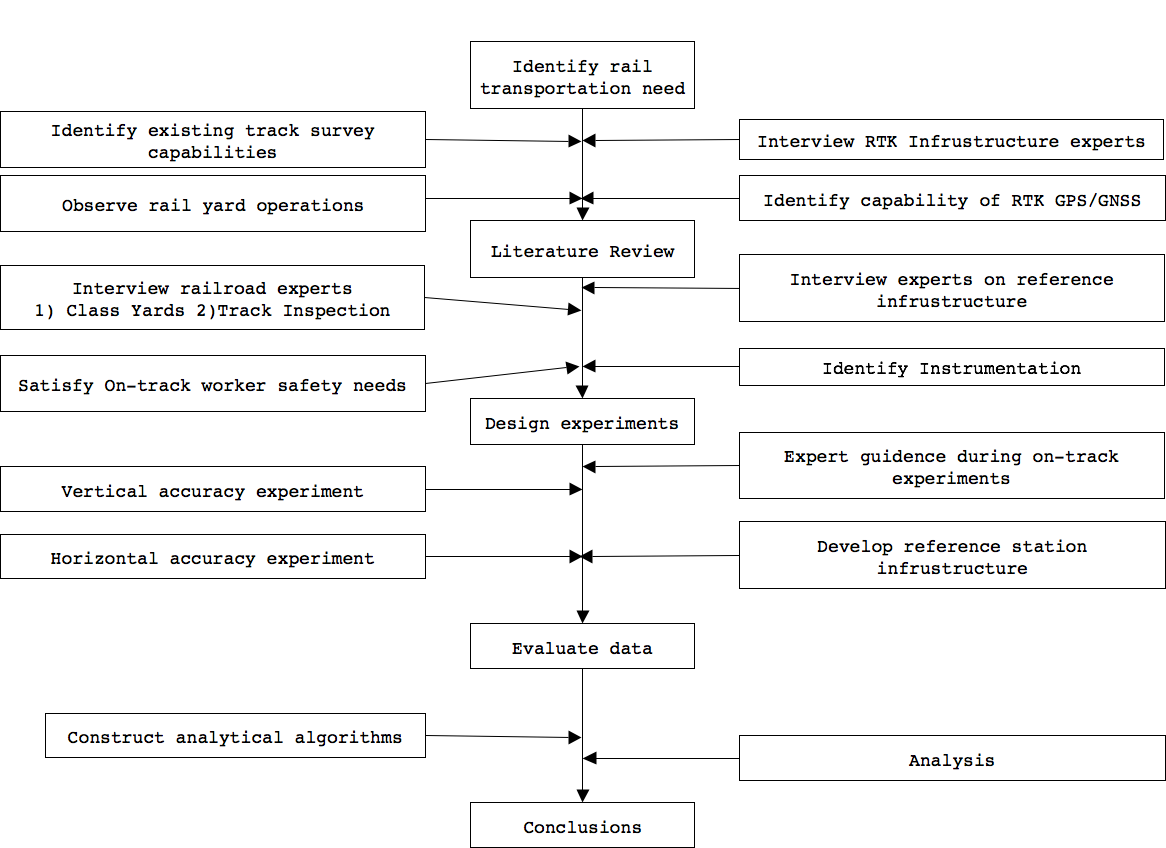
\includegraphics[width=6in]{graphics/research_plan.png}
	\caption{Research Plan}
	\label{fig:plan}
\end{figure}
The research investigated the capabilities of RTK GPS/GNSS over active track. Due to federal and private property laws restricting access to active track, all research activities were performed adhering to the provisions of 49 CFR \S214 railroad workplace safety regulations, subpart C \textit{Roadway Worker Protection}~\citep{49CFR214300} and subpart D \textit{On Track Roadway Maintenance Machines and Hi-Rail Vehicles}~\citep{49CFR214500} as well as specific rail company rules and procedures set out by the employee in charge during job safety briefings. 

Track location of bowl tracks in a hump yard was determined from single epoch track observations from a GPS mounted on a locomotive traversing an active hump yard. The track positions were used to produce profiles for each bowl track in the yard. Relative vertical precision and base station observations were used to evaluate the yard environment for RTK GPS surveying by locomotive.

An evaluation of RTK augmented horizontal performance was made by single epoch observations of track position by RTK GNSS receivers mounted to a track inspector's Hi-Rail traversing active mainline track. Horizontal track alinement was evaluated by means of a software modeling the string lining method to determine the degree of curve from single epoch RTK GNSS track position observations. Degree of curve ($D_c$) determined by the RTK GNSS string line model was compared with $D_c$ determined by a track geometry car over an identical tangent segment.

An evaluation of RTK GNSS to determine track occupancy was made by multiple Hi-Rail traverses with RTK GNSS instruments across multiple parallel segments of mainline track. Positions observed over identical and parallel segments of tangent and circular track were evaluated for cross-track error\footnote{per Allen et al., \pageref{fig:trackRef}} for the likelihood of determining track occupancy by an RTK GNSS equipped mobile rail vehicle.

The electrical point of reference for a GPS/GNSS antenna is the phase center. The phase center is offset some distance from a physical reference location on the antenna housing. The physical antenna reference for each of these experiments was the mounting surface or antenna reference point (ARP). The survey controller contains a table of offset distances between phase center and ARP for the antennas used during each experiment. A procedure to align the ARP on the track vehicle to a selected railway reference location\footnote{i.e., Track centerline, left (port) gauge side or right (starboard) rail.} was performed as part of the mobile track vehicle setup.

Estimates for the relative horizontal and vertical precision\footnote{Relative errors are errors and precisions expressed for and between pairs of network adjusted control points.} are calculated by the \emph{Survey Controller} software in the Trimble TSC2 controller. \emph{Trimble Survey Controller} software uses a algorithm to compute vertical precision:
	\begin{equation}
Vertical Precision (m) = ErrorScale * VDOP * ScaleFactor\\
	\end{equation}
Where:\\
${ErrorScale = \frac{\sqrt{ErrorE + ErrorN + ErrorU}}{PDOP}}$\\
ErrorE = CovENU[x][x]\\
ErrorN = CovENU[y][y]\\
ErrorU = CovENU[z][z]\\

Where CovENU is the aposteriori covariance matrix of the RTK solution from the RTK engine in the GNSS receiver.\\
\emph{ScaleFactor} is either 1 or 1/3 depending on whether the RTK engine is giving \emph{Survey Controller} 1-sigma or 3-sigma precisions, which depends on the version of RTK engine. The \emph{Survey Controller} display shows 1-sigma precisions.\\

The observation procedure for these experiments progress from setup of an ad hoc  reference station in the case of experiment 1, or accessing a VRS reference network as in experiments 2 and 3; establishing a means of communication between the reference station/VRS and the track vehicle; aligning the antenna with a track reference point; and configuring the mobile receiver onboard the track vehicle.

%Hump yard profile design
\subsection{Experiment One: Hump Yard Profile Survey} \label{ResDHmpYd}

Experiment one asked whether RTK augmented GPS mounted to a locomotive could measure the  vertical profile of bowl tracks in an automatic classification yard without the need for track closures.

The objective of experiment one was to use RTK GPS instrumentation mounted to a locomotive to survey an active hump yard in order to produce track profiles. The survey data was used to create information products which were handed off to the rail company sponsor in preparation for a yard-wide resurfacing project.
%{Ad Hoc Base Station Procedure}

Coordinates are reported as in US survey feet,
\begin{description}
	\item System: US State Plane 1983.
	\item Zone: North Carolina 3200
	\item Datum: North American Datum 1983
	\item Geoid: Continental United States 2003
\end{description}

The hump yard survey used a single RTK reference station transmitting correctors via UHF radio to a mobile receiver onboard a locomotive.  The ad hoc reference station components are listed in table \ref{tab:instruments}. A fixed-height tripod at 1.5 meters supported the GPS and UHF antennas. The ad hoc reference station was set on top of a two story masonry structure to maximize height above average terrain (HAAT) for UHF data reception by the roving receiver aboard the locomotive as shown in figure figure \ref{fig:AhRS}. The elevated location provided sufficient HAAT to enable reception of correctors across the yard and to NGS benchmark EB1559 located 8,500 feet from the 25 watt UHF transmitter.

The autonomous horizontal position of the reference station (CP1) was adjusted by using the results of NGS OPUS from observations recorded during two sessions. The first session was 2008/05/26 14:21:00 to 21:44:00 UTC with the second session 2008/05/27 12:12:00 to 18:50:00 UTC\label{baseRefPeriod}. The compressed observation files were converted\footnote{Using Trimble \emph{runpkr00} under Unix.} to the Receiver INdependent EXchange (RINEX) format and submitted to the National Geodetic Survey Online Position User Service (NGS OPUS) for position determination. The autonomous horizontal position of the ad hoc reference station (CP1) was adjusted to the mean northing and easting of the two NGS OPUS reports exhibited in Appendix A, pages \pageref{opus1}-\pageref{opus2}.

The autonomous vertical position of the reference station was adjusted using RTK observations on a NGS benchmark, permanent identifier (PID) EB1559. The benchmark was located 8,508 from the ad hoc RTK reference station. The elevation of CP1 was adjusted to minimize the difference between the observed and the published NAVD88 elevation for the first order class II\footnote{\citep{FGCCstds}} benchmark. The PID datasheet for EB1559 is exhibited in Appendix A, pages \pageref{EB1559-1}~-~\pageref{EB1559-3}.

Multipath concerns were examined at the reference stations by generating a full TEQC~\citep{TEQCsoftware} (Translation, Editing, and Quality Check) report from the reference station RINEX observation and navigation files. The TEQC reports are exhibited in Appendix A.

% AhRS setup photo
\begin{figure}[!h]
  \begin{center}
    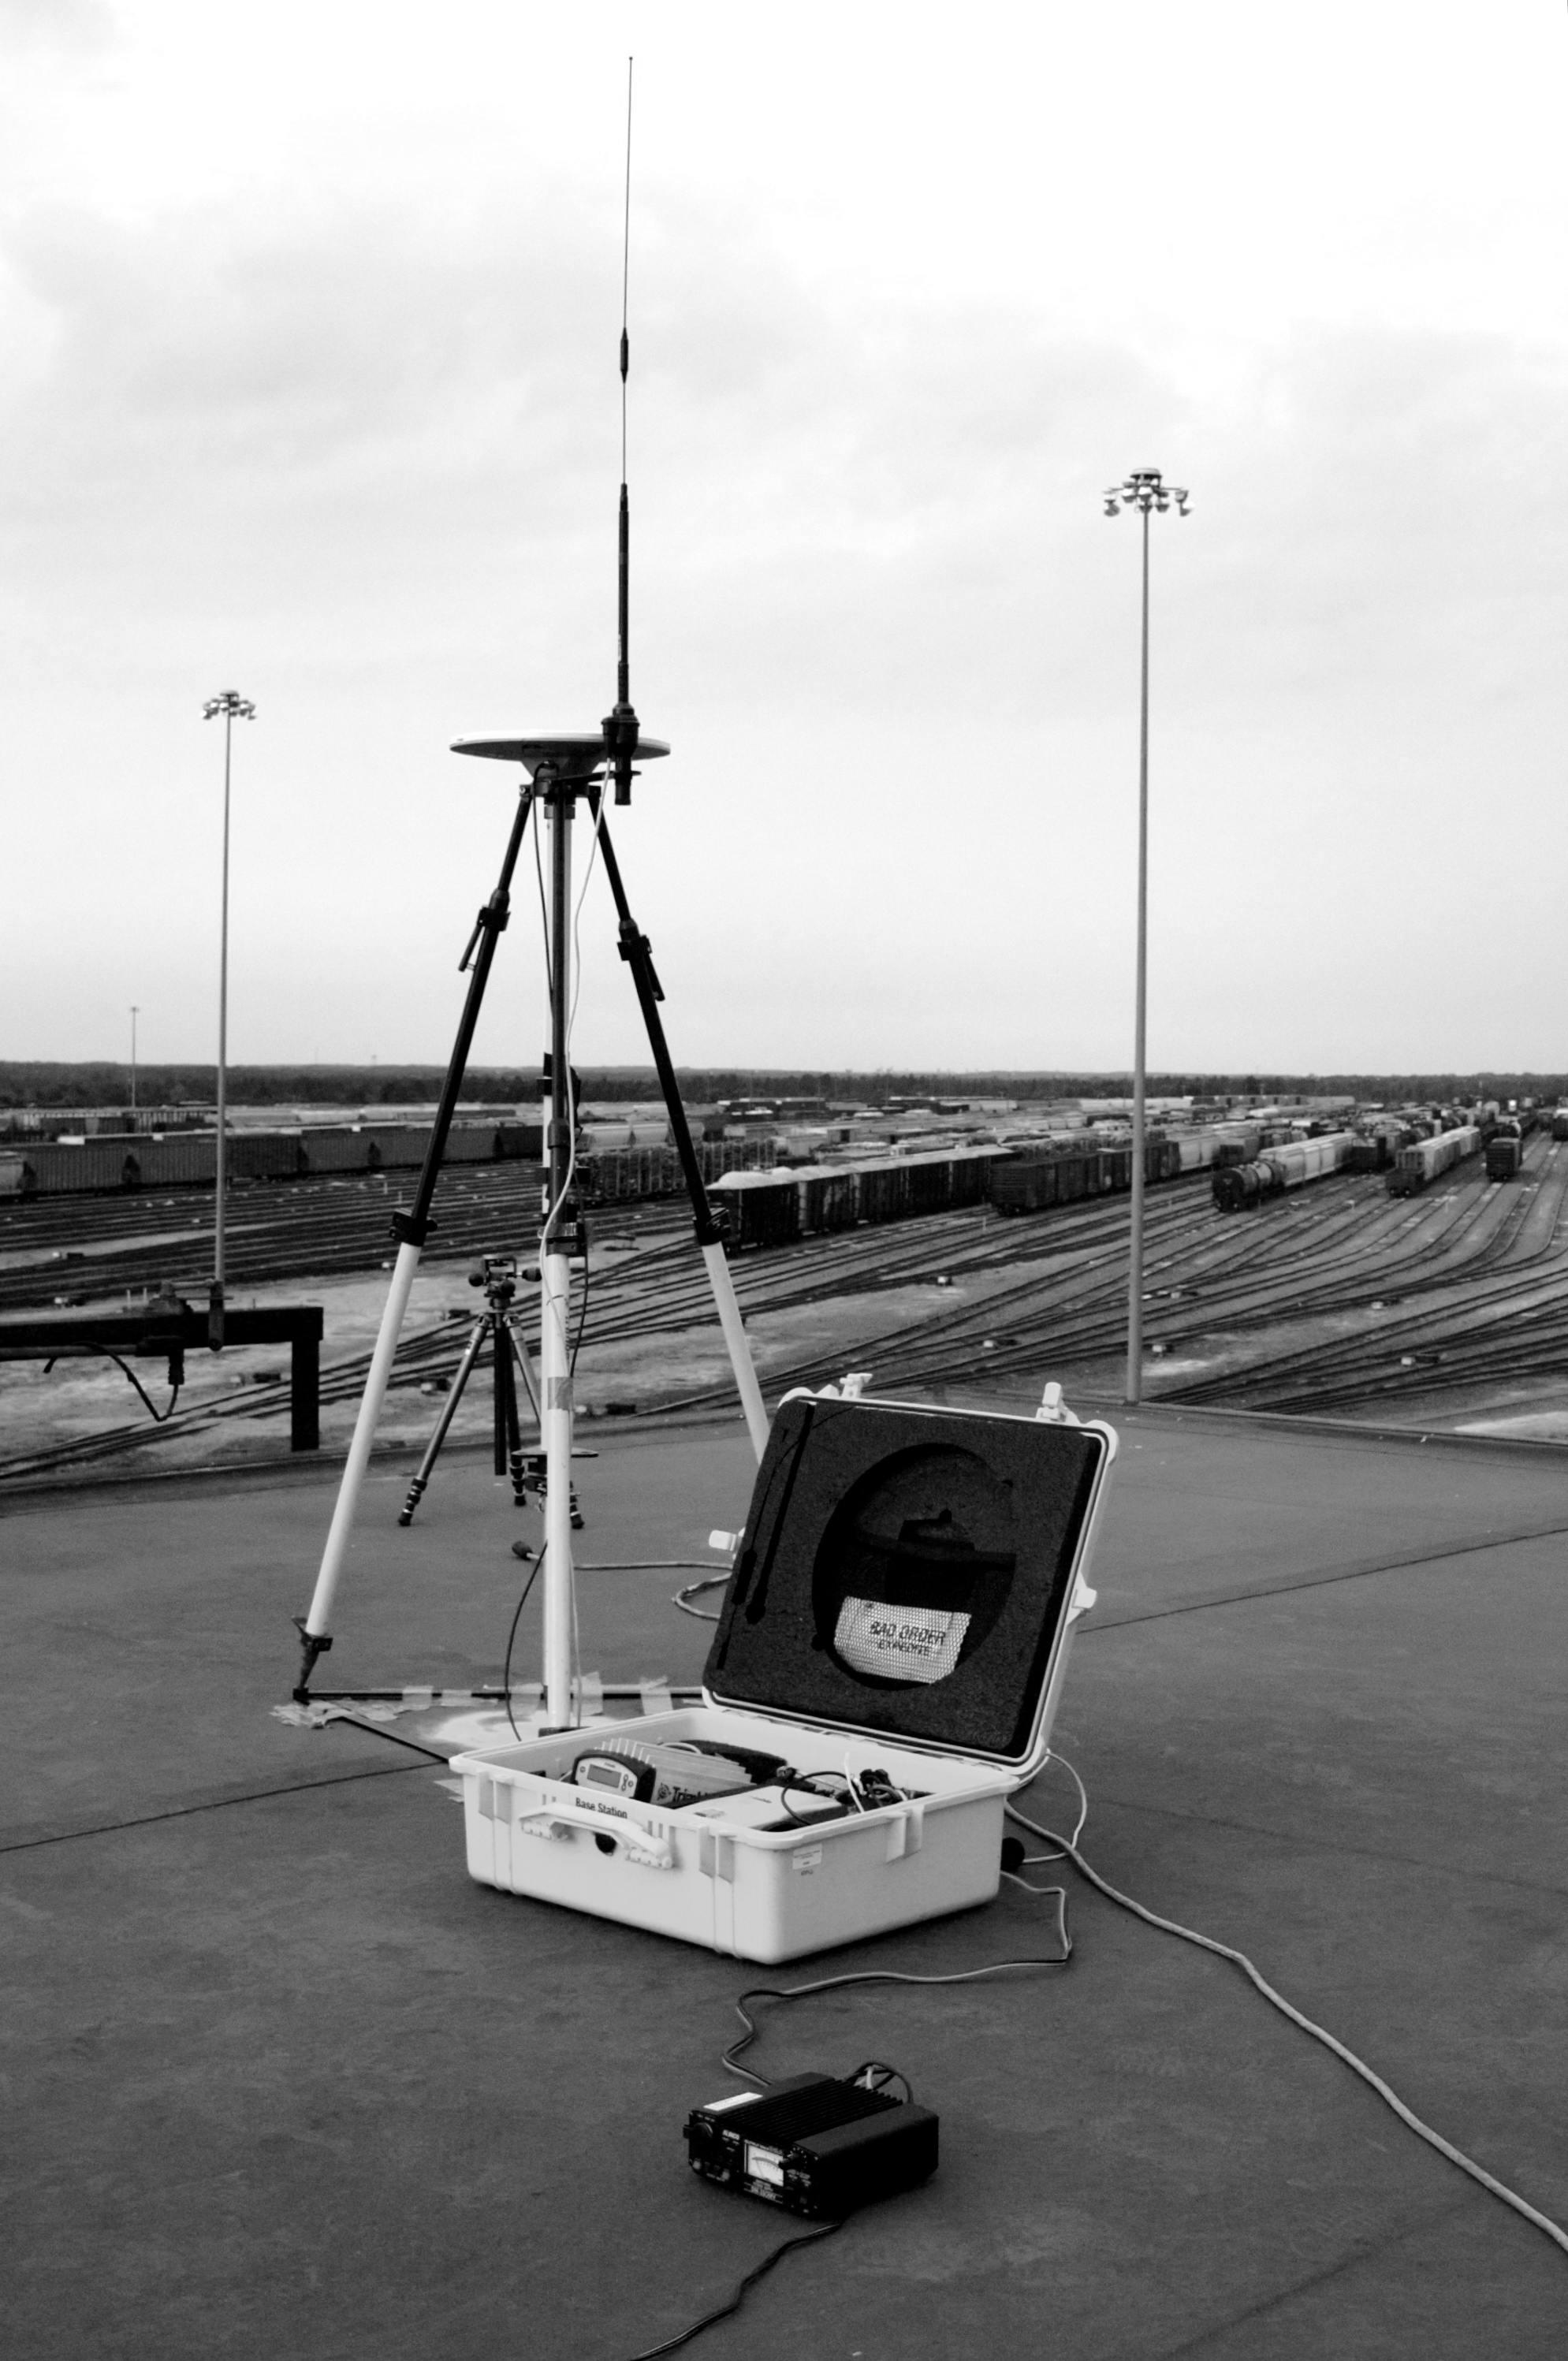
\includegraphics[scale=0.5]{graphics/AhRS_hamlet_BW}
   \caption{Ad hoc Reference Station}
  \label{fig:AhRS}
\end{center}
\end{figure}

An EMD SD60 yard locomotive was equipped with the mobile\#1 instrument indicated in table \ref{tab:instruments}. The mobile GPS antenna mount was collocated with an omnidirectional UHF antenna and secured to a SECO magnetic base as illustrated in figure \ref{fig:locoAnt}. The antenna mount was fitted with a wire rope safety lead to secure the antenna assembly to a fixed member on the locomotive cab to prevented injury to locomotive operators or ground personnel in the event the antenna was dislodged by handling rail cars. The antenna were  connected to the mobile receiver with ten-foot lengths of RG-58 50\ohm~coaxial cable.

% AhRS setup photo
\begin{figure}[h!]
  \begin{center}
    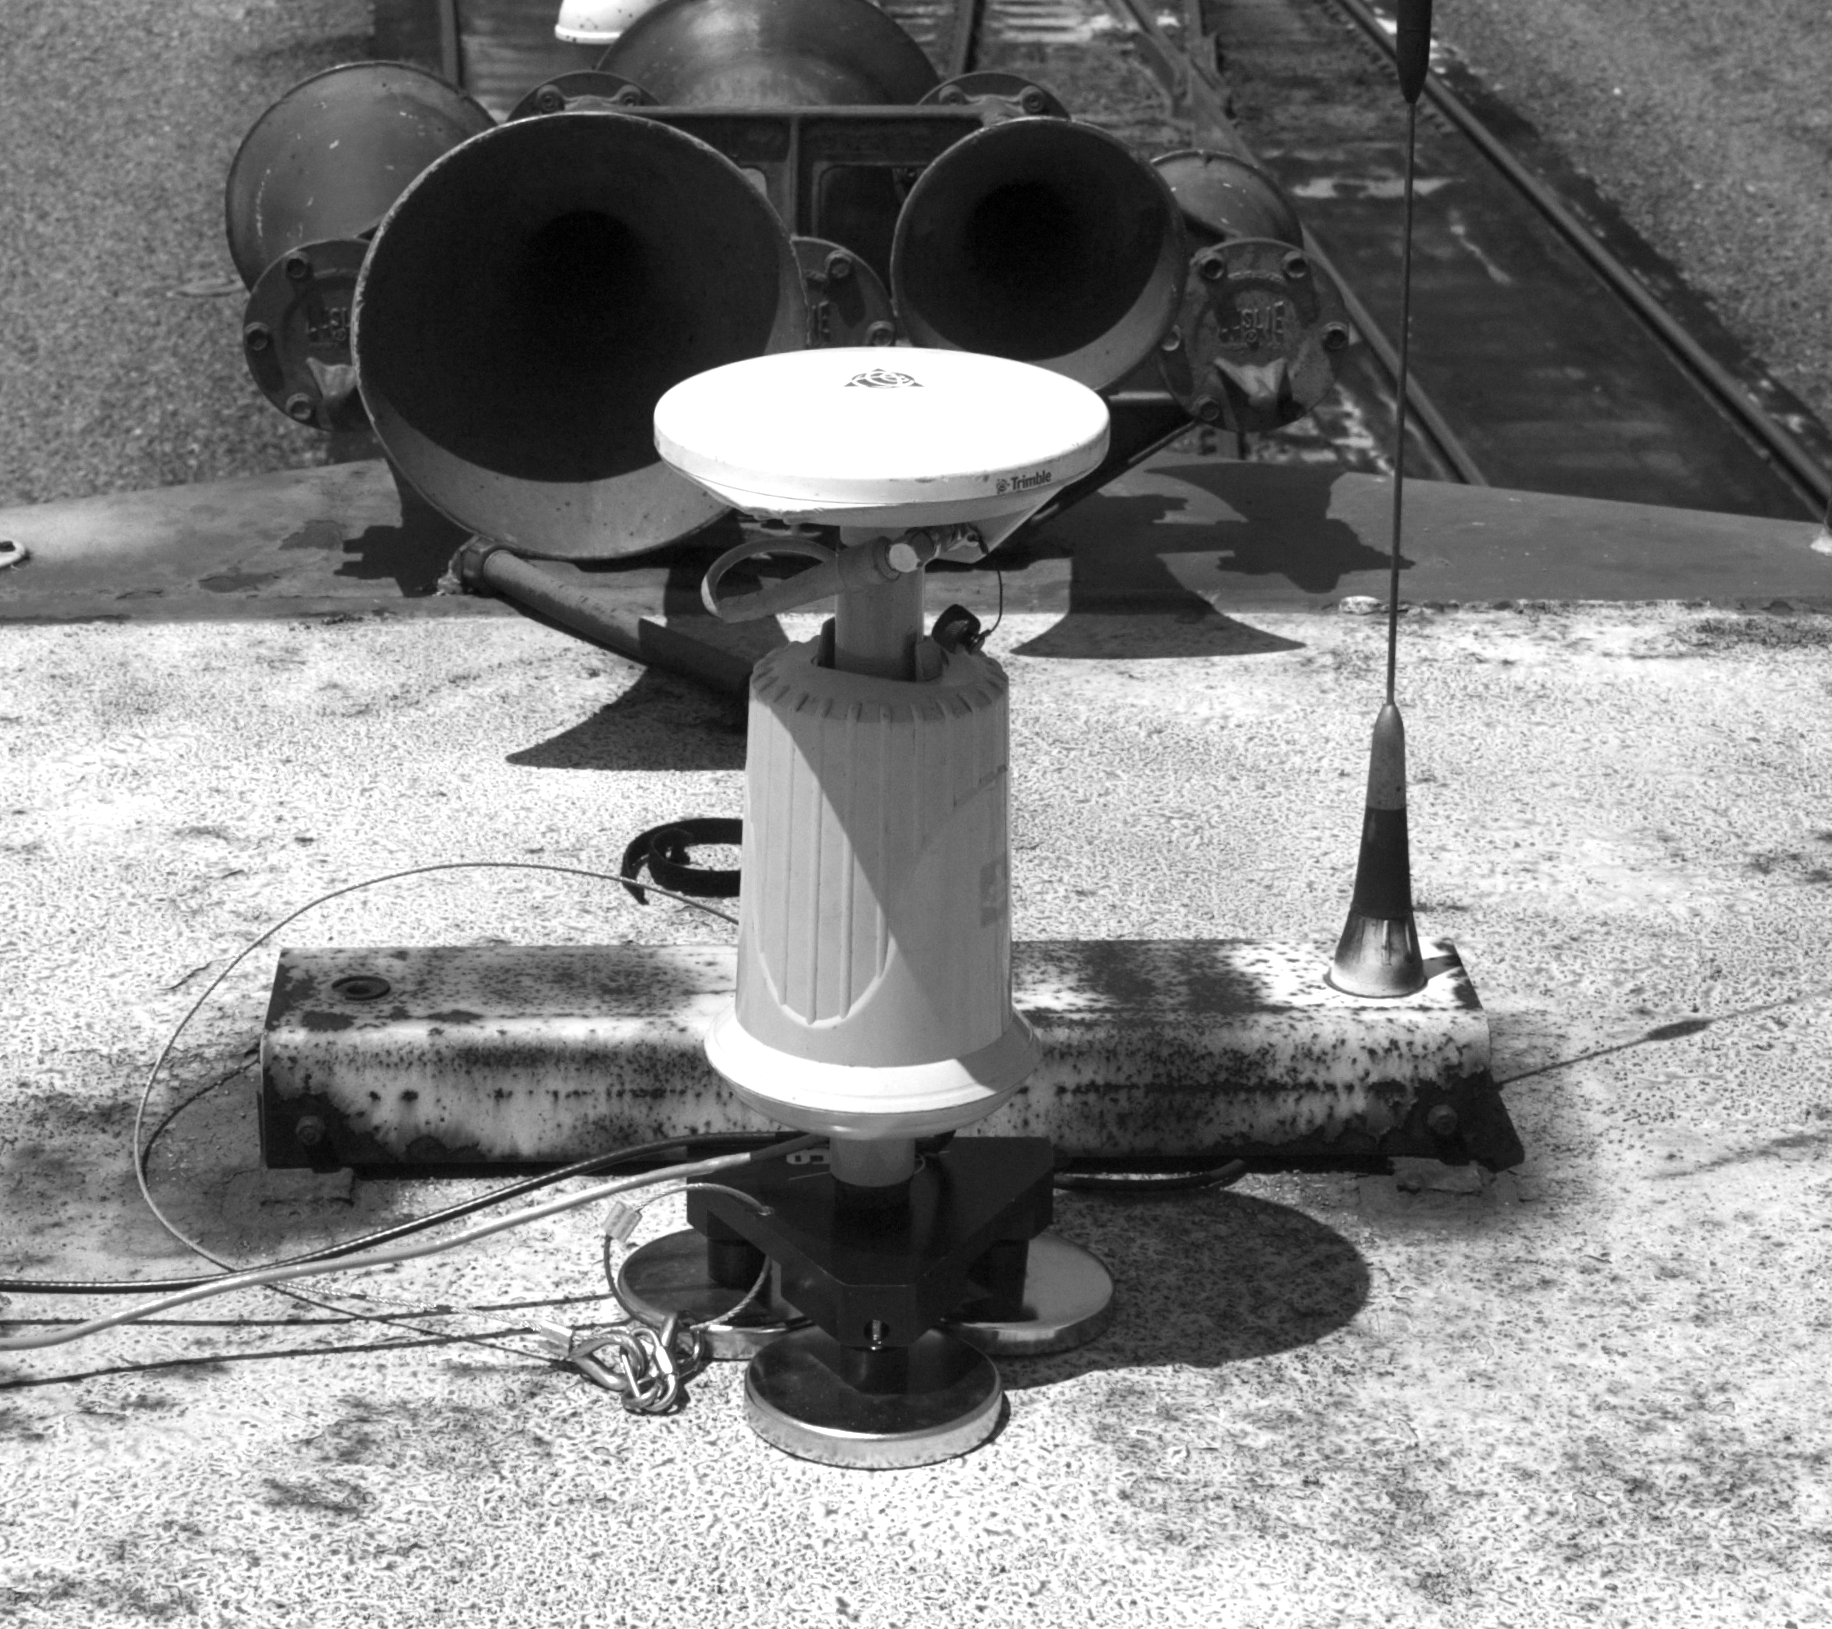
\includegraphics[width=0.48\textwidth]{graphics/AntennaMountBWcrop}
  \end{center}
  \caption{GPS/UHF Antenna Setup on Locomotive}
  \label{fig:locoAnt}
\vspace{-20pt}

\end{figure}
The antenna was aligned with the track centerline in an area designated by the yardmaster and blue flagged during installation to insure the safety of research and railroad company personnel working around the locomotive. The generalized procedure for aligning a GPS/GNSS antenna mounted to a track vehicle with a horizontal track reference and determining the antenna reference point from the top-of-rail elevation is described following and referencing figure~\ref{fig:antAlign}.

% Antenna alignment procedure
\subsubsection{Antenna Alignment Procedure}
\label{Antenna Alignment}
\begin{enumerate}
\item A job safety briefing is conducted by the rail company employee-in-charge.
\item A frequency in the 450~Mhz band is selected by monitoring voice traffic on available channels, as data is a secondary use of this spectrum. The ad hoc reference station is programed with an autonomous position, and corrector transmission initiated.
\item  A section of tangent track approximately 300 feet long is blue flagged and made safe by setting a derail and locking out the track switch as discussed during the job safety briefing.
\item Track centerline points are measured on either end of the calibration area, figure~\ref{fig:antAlign} points A and A'. The centerline points are observed with a Trimble R8 instrument for 180 epochs.
\item A line feature representing the track centerline is created in the survey controller between points A and A'.
\item The center point of the line feature is determined. Two points, referenced in figure~\ref{fig:antAlign} as points B and B', are observed at the the top of each rail for 180 epochs.
\item A second line feature between points B and B' is created in the survey controller.
\item A point located by intersecting lines A-A' and B-B', figure~\ref{fig:antAlign} point C, is determined by the \emph{Survey Controller} software.
\item The mean elevation of the top of rail observations is calculated and assigned to point C.
\item The GPS/UHF antennas and magnetic base mount are placed in the approximate center of the top of the locomotive cab. A wire rope safety harness connecting the antenna mount to the locomotive horn or other suitable anchor point is secured.
\item The survey controller is connected to the GPS receiver in the track vehicle. The previously created data file with the alignment features described above is opened.
\item Blue flags are removed from the locomotive by the persons that placed them. Derails are stowed and facing point track switch operators are unlocked. Movement authority is obtained from the yardmaster by the locomotive engineer.
\item The locomotive is moved to locate the GPS/UHF antenna mount over point C.
\item The locomotive is secured and the antenna mount moved in small increments to intersect the centerline by observing the instantaneous antenna location in the map view of the controller. A period of  ten seconds between movements is allowed for the position to settle in the map display.
\item The survey controller antenna height is set to zero. Figure~\ref{fig:antAlign} point D is observed for 180-epochs. An inverse calculation is performed between points C and D. The elevation difference is recorded as the antenna height.
\item A survey style is created in the \emph{Survey Controller} software containing the antenna height above the top-of-rail elevation. Due to variation in cab height above top-of-rail, the survey style is named for the particular locomotive unit number used in the antenna alignment. Likewise for individual Hi-Rail vehicles.
\end{enumerate}

% Alinement drawing
\begin{figure}[h!]
  \begin{center}
    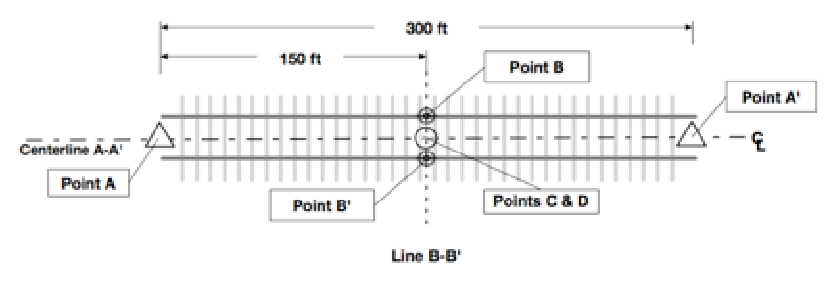
\includegraphics[scale=0.40]{graphics/antennaAlinement.png}
  \end{center}
  \caption{Track Vehicle Antenna Alinement Procedure}
  \label{fig:antAlign}
\vspace{-20pt}
\end{figure}

RTK correctors were broadcast from the single reference station by UHF data radio and used to augment the GPS receiver aboard the locomotive. A survey controller connected to the receiver managed and automated data collection by recording single epoch observations with a nominal horizontal separation of ten feet. Track profiles originated at a common reference point at the hump end of the bowl and terminated at the pullout-end switch for each track.

The pullout end of the bowl was surveyed first, from pullout switch to foul point\footnote{The track foul point is the demarcation between hump and pullout end movement authority.}. The hump end of the bowl was surveyed during a shift change, from the hump to foul point, to minimize disruption to humping operations. Locomotive movement across the pullout end of the yard was coordinated between the locomotive operator and pullout end humpmaster\footnote{Responsible for outgoing train makeup and movement.}. Track traverses began at the pullout end switch and progressed to the foul point. The automatic numeric sequencing of the survey controller was used to produce unique point identifiers. The controller sequence was constructed by concatenating: 1) the  two digit track number; 2) a single digit traverse counter; 3) a three digit point sequence beginning at 000 and incremented by one at each observation in sequence. Points recorded onboard the locomotive were feature coded as centerlines.

The hump end survey was performed in coordination with the hump end humpmaster\footnote{Responsible for railcar sequencing and switching into the bowl.} during the yard shift change to minimize the impact of the survey interrupting yard production. The locomotive traverse of the hump end began at the hump, through the retarder and track leads, finishing at the track foul point. The unique point identification scheme previously described was not performed due to time constraints. The hump, leads, and track points were separated post survey.

Points of interest (POI) were surveyed on the ground with the static module referenced in table \ref{tab:instruments}. The static receiver was mounted to a 2 meter range pole. Multiple epoch observations (3-6) were recorded at each point of interest. Feature codes distinguished switch points, wheel detectors, retarder inlet/outlet, and foul points. Switch points and retarders were identified by rail company reference number. Wheel detectors were identified by track and sequence number. Ground point safety was superintended by a rail company employee.

% Hump Yard Data
\emph{Variables of analysis}: The mobile instrument \#1, table \ref{tab:inst} produced these variables:
\begin{itemize*}
\firmlist	
	\item US State Plane, North Carolina 3200, northing in US survey feet.
	\item US State Plane, North Carolina 3200, easting in US survey feet.
	\item NAVD 88, height above ellipsoid 2003, in US survey feet.
	\item Vertical precision estimate determined by \emph{Survey Controller} software, in US survey feet.
	\item Time (local, EST) and date of observation.
	\item A count of the SVs in view of the mobile\#1 GPS antenna.
	\item Vertical Dilution of Precision (VDOP)\footnote{A unitless figure of merit expressing the relationship between error in in user position, and the error in satellite position. PDOP is related to the horizontal and vertical PDOP by: ${PDOP = \sqrt{HDOP^2 + VDOP^2.}}$} determined by \emph{Survey Controller software}
\end{itemize*}

Yard observations were exported from the \emph{Survey Controller} software and separated into layers organized by lead, group, and track. Deconstructing the aggregate observations enabled individual tracks to be configured as a continuous series of points by activating the particular layers in TGO.
\begin{itemize}
\item Hump lead
\item Main retarder
\item Intermediate retarders
\item Group retarders
\item Group leads
\item Bowl tracks
\end{itemize}
A properly configured track was apparent as a continuous series of points extending from the hump through the desired track to the pullout end switch.

Locations of track POI (i.e., track switch points, retarder inlet and outlet, wheel detectors) were associated with a position nearest a particular rail. The POI was observed at the center top-of-rail nearest the POI physical location using the static survey instrument. The position of each POI was adjusted post survey to be coincident with the track centerline.

Continuous track observation names were renumbered in the TGO software, in series progressing from hump to pull out. Feature codes enabled separation by feature. The \emph{TGO} software was used to create line work by connecting consecutive centerline points. The line work and observation data were exported from TGO in the ESRI\footnote{Environmental Systems Research Institute, Inc.} shapefile format. The point data was also exported as a comma delimited (CSV) format and imported to a \emph{Google Docs} spreadsheet. A linear reference was determined for each point according to equation \ref{eq:horzSta}. Elevations and linear references were scaled and input as an overlay to a CAD drawing containing the track design grade\footnote{Provided by the rail company sponsor.}. 

Each track profile was plotted as an overlay to the provided CAD drawing. The design profile in the CAD drawing is relevant to the rail company in a making a volumetric assessment of surfacing material required to bring the relief of each track into vertical alignment with the design grade. Calculation of surfacing material quantity is outside the scope of the experiment. The design grade and locomotive survey result will be used as a comparative tool, limited to providing track profile deviation from design grade.

The shapefiles will be added to ESRI ArcMap software where a plan view of of the bowl area track elevation and vertical precision estimate will be represented in plan view. The vertical precision map will show lower quality vertical precision for points > 0.1 feet in a contrasting color to those of greater precision. The plot will be examined for the distribution of lower quality data patterns.

Acceptable elevation quality will be apparent as a smooth track profile. Poor quality observations will appear with greater variation between points, resulting in a jagged or sawtooth profile. Poor quality elevations will be identified and correlated with: observation time; vertical precision estimated by the receiver; and reference station observations during the period.

The vertical precision calculated by the \emph{Survey Controller} software was used to determine descriptive statistics and to plot a histogram for analysing the quality of GPS observations by the mobile instruments.

%Horizontal stationing equation
	\begin{equation}
	{sta_k} = {match~point~offset} + {\sum_{k=2}^n}  {\sqrt{(x_k - x_{k-1})^2 +( y_k - y_{k-1})^2}}
	\label{eq:horzSta}
	\end{equation}
\begin{quotation}
Where \emph{k} =  a point in the ordered sequence of observations, and \emph{n} = the number of observations in the track segment, and the match point offset is the horizontal distance from the top of the hump to switch point 1574.
\end{quotation}

Experiment one:
\begin{enumerate}
	\item Produced an alignment procedure for alignment of the GPS antenna with the centerline top-of-rail location.
	\item  Collected continuous single epoch observations on a nominal 10 foot horizontal spacing with RTK augmented GPS onboard a locomotive in an active hump yard. 
	\item Resulted in the production of a plan-view color-map of track elevation for the bowl area of a hump yard.
	\item Resulted in the production of a plan-view color-map of relative vertical precision as determined by the \emph{Survey Controller} software for points measured in the bowl area of the yard.
	\item Resulted in the production of a two-dimensional profile drawings for each track in 1:1 and 1:5 vertical scale.
	\item Determined the descriptive statistics of the relative vertical precision as determined by the \emph{Survey Controller} software for the locomotive mounted GPS .
	\item Resulted in the production of TEQC reports for two ad hoc reference station observation sessions.
\end{enumerate}

% Mainline Track alinement design
\subsection{Experiment Two: Determining Horizontal Track Alinement}
\label{Ex2Design}
This research asks whether RTK augmented GPS and GNSS instruments mounted to a common track vehicle can determine horizontal track alinement comparable those acheived by specialized track geometry vehicles. The objective of the experiment was to perform multiple mainline track surveys with RTK instruments mounted to a Hi-Rail vehicle; the development and demonstration of a software model using the string lining procedure in order to produce horizontal track alinement. The track alinement survey employed a series of CORS RTK reference stations along the survey route, networked to the Ohio Department of Transportation, Aerial Mapping Virtual Reference Station (ODOT VRS) server.

The ODOT VRS was used to minimize the $\pm$1 ppm error incurred as distance increases from a reference station. The VRS creates a new virtual reference station when the baseline between the track vehicle and the previous VRS created reference station increased beyond a distance programmed in the VRS. A public cellular data service was used to exchange security credentials with  the ODOT VRS server, receive correctors, and apply them to a mobile receiver onboard a track inspector's Hi-Rail. A survey controller connected to the mobile receiver recorded single epoch observations with a nominal horizontal point separation of five feet with mobile instrument\#2 (table \ref{tab:instruments}) and ten feet with mobile instrument\#1. Nominal point separation was based on the receiver processing speed for Hi-Rail traverses in the range of 10 to 30 mph.

% Alinement Study Area
Two mainline track segments of different character were traversed during this experiment. The first segment can be characterized as multiple parallel track, signalized, Class 4, with a maximum allowable track speed between 30 and 50 mph, carrying a freight volume of 25 to 35 MGT/yr\footnote{Million Gross Tons per year}. This segment is referenced as C\&O Kanawha subdivision, from mile post 494 to 523 (MP494-523). Continuous observations over this segment demonstrates the capability of an RTK VRS over a wide area.

A second segment, characterized as single track, dark territory, Class 3, with allowable track speed between 10-30 mph, carrying a freight volume of less than 10 MGT/yr, is referenced as C\&O Ohio River subdivision from mile post 210 to 207 (MP210-207). This segment was selected for study as the segment had been examined previously by Szwilski~\citep{Szwilski03}. Additionally, data was made available from CSX's Gauge Restraint Measurement System\footnote{A specialized, self-propelled, track geometry car.} (GMRS) across this segment. Degree of curvature (${D_c}$) from the GMRS was compared with the horizontal alinement model by selecting a tangent segment for comparision. An ideal measurement across a tangent segment would result in a ${D_c}$ of zero. Therefore, the ${D_c}$ deviation from zero across the tangent segment was used to compare the GMRS measurement with RTK modeled ${D_c}$ measurements.

% FRA alinement figure
\begin{figure}[!htp]
	\vspace{-30pt}
		\begin{center}
			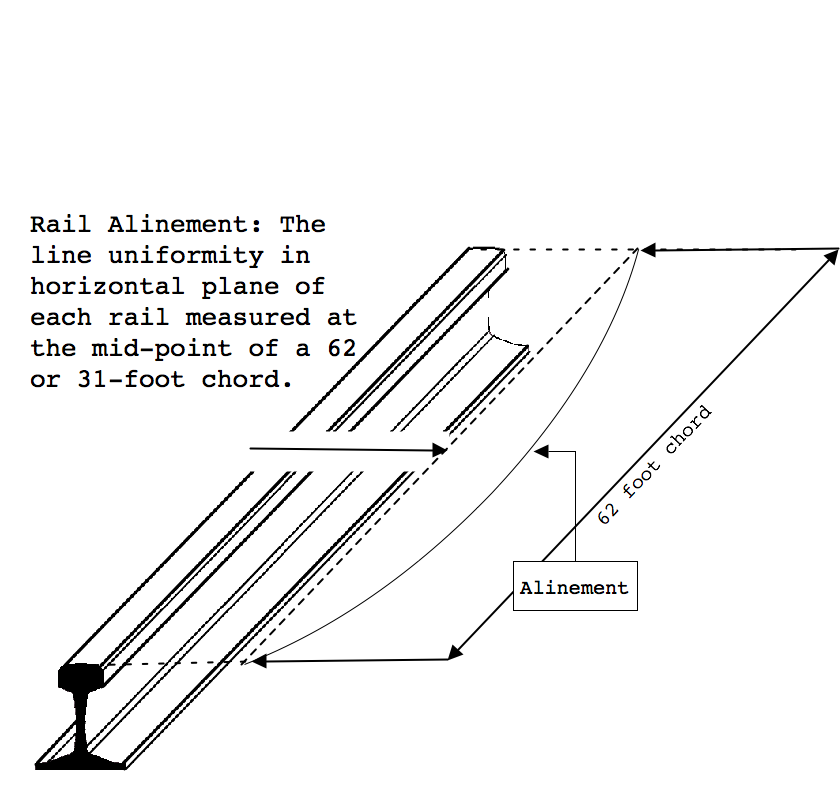
\includegraphics[width=3in]{graphics/HorzAlignment.png}
			\caption{Horizontal Alinement}\label{fig:Alinement}
		\end{center}
	\vspace{-30pt}
\end{figure}

The track observations were used as inputs to a software to determine the ${D_c}$ modeling the FRA guidance manual instructions for using the string line method.
Experiment two objectives sought to:
\begin{enumerate}
	\item Collect continuous single epoch observations with RTK augmented GPS/GNSS mounted to a track inspector's Hi-Rail over at least 29 continuous miles of mainline track. Point spacing was a nominal 10 foot for mobile configuration\#1 and 5 foot horizontal spacing for mobile configuration \#2 (see table \ref{instruments}).
	\item Develop a software model for calculating degree of curvature (${D_c}$) from RTK augmented GPS/GNSS track vehicle observations. The software model replicated the string lining method described in FRA \emph{Track Safety Standards Compliance Manual}~\citep[pp.26-30]{2007FRATrack} using a 62 foot chord length and 15.5 foot stations.
	\item Compare two methods of measuring ${D_c}$ over tangent track. The first method utilized data from a specialized track geometry car, CSX's GMRS. The self propelled GMRS was designed specifically for the purpose of obtaining ${D_c}$ (and other track alinement parameters\footnote{Gage, crosslevel, profile, ${D_c}$}) from the string lining method. The second method utilized data obtained from an RTK GNSS instrument mounted to a track inspector's Hi-Rail and a software to model the string line method from the Hi-Rail data.
	A traverse of identical tangent track segments was compared for cross-track\footnote{See Allen, et al., figure \ref{fig:trackRef}, page \pageref{fig:trackRef}} centerline deviation using descriptive statistics. Identical segments were determined by selecting beginning and ending mile post reference locations.
	\item The ${D_c}$ was determined and track elevation measured using RTK survey equipment mounted to a track inspector's Hi-Rail across a continuous 29 mile track segment. The modeled ${D_c}$ was compared with company supplied track charts to correlate the location and magnitude of curves. Structures responsible for loss of signal (LOS) were identified.
\end{enumerate}

\emph{Variables of analysis}: The mobile instrument \#1 and \#2, table \ref{tab:inst} produced these variables:
\begin{itemize*}
	\item UTM, Zone 17 North, northing in US survey feet.
	\item UTM, Zone 17 North, easting in US survey feet.
	\item NAVD 88, height above ellipsoid 2003, in US survey feet.
	\item Time (local, EST) and date of observation.
\end{itemize*}
\emph{Variables of analysis}: The CSX GMRS produced these variables of analysis:
\begin{itemize*}
	\item Mile post offset distance, in feet.
	\item Degree of curve, 62 foot chord, in degrees.
\end{itemize*}

%Data Collection Experiment 2

The mobile antenna (table \ref{tab:instruments} mobile~\#2) was alined using the generalized procedure listed on page \pageref{Antenna Alignment}, and mounted to a track inspector's Hi-Rail vehicle as illustrated in figure \ref{fig:antHi-Rail}. The receiver was programmed to process observations in ``low latency'' mode, which uses approximately 20 milliseconds to compute each observation, degrading the manufacture's stated horizontal accuracy of $\pm$~1~cm by an additional centimeter~\cite[pp.8]{Trimble5700}~\cite[pp.9]{TrimbleR7gnss}.

% Hi-Rail antenna
\begin{figure}[h!]
  \begin{center}
    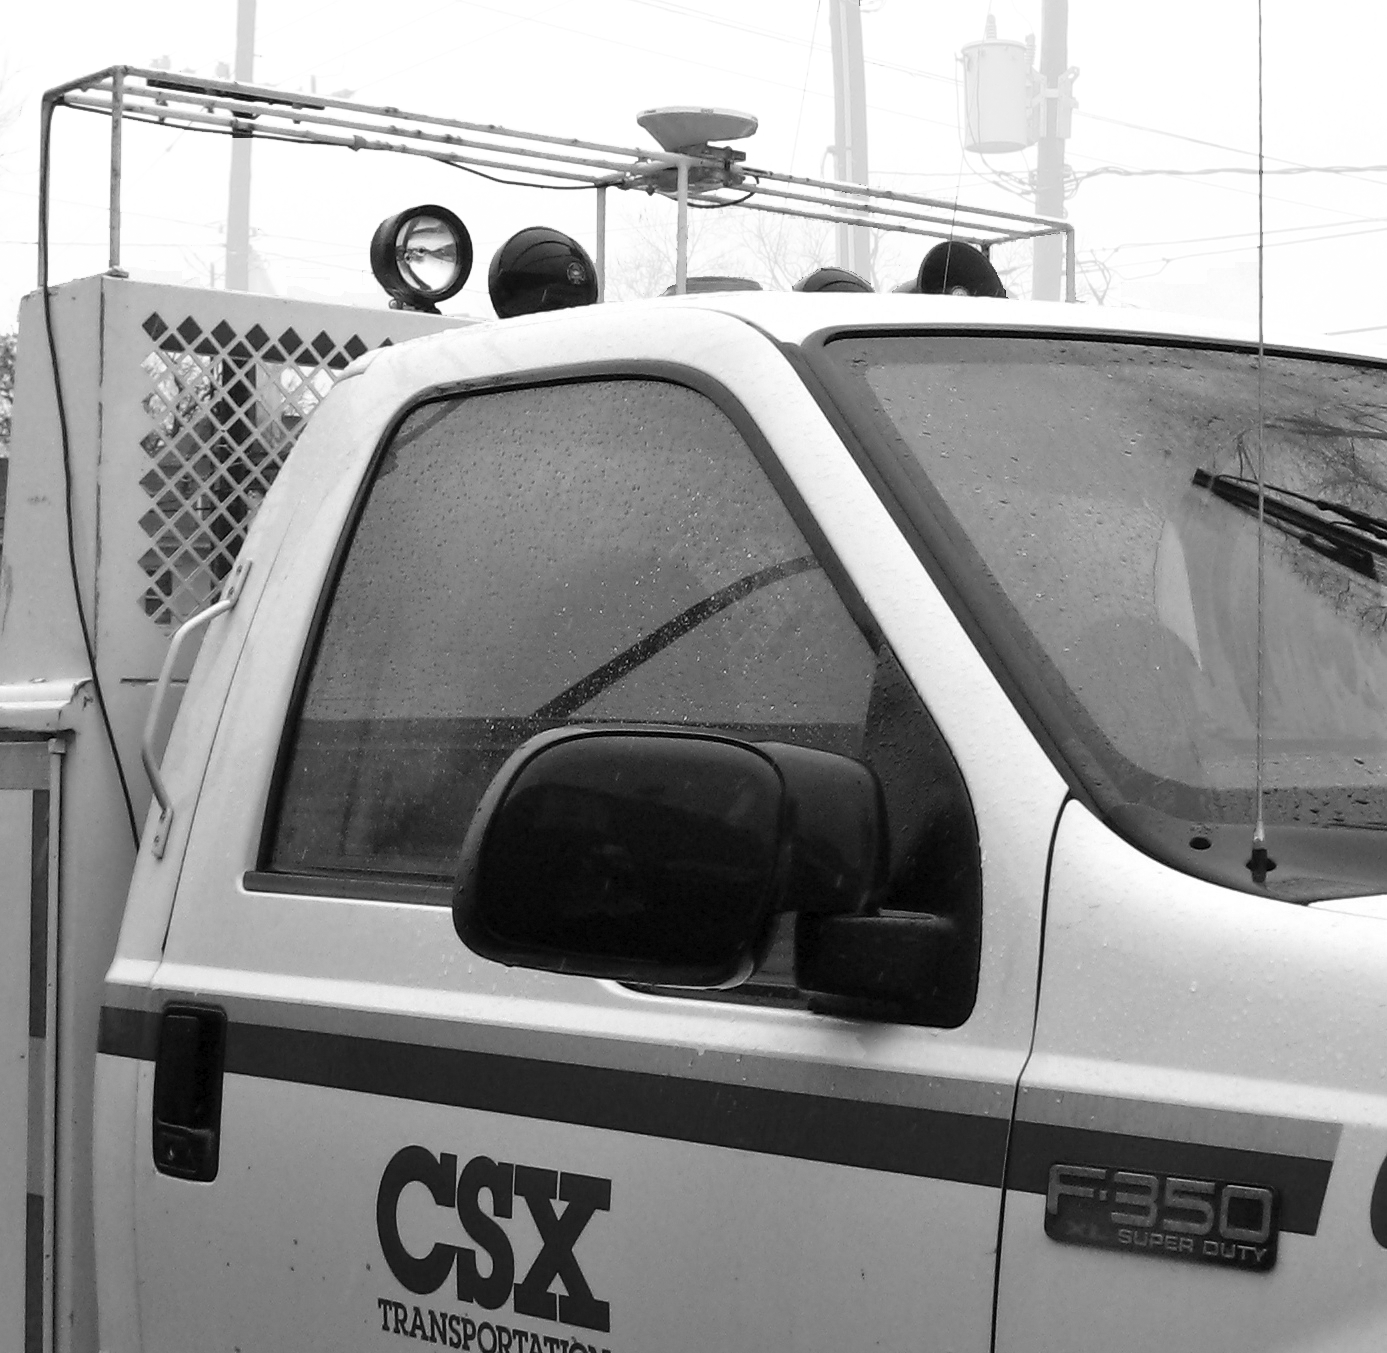
\includegraphics[scale=0.50]{graphics/HiRailAnt_modBW.png}
  \end{center}
  \caption{GNSS Antenna Mount, Hi-Rail}
  \label{fig:antHi-Rail}
\vspace{-20pt}
\end{figure}

The controller was programmed to collect observations on a nominal 5 foot spacing. Mile post centerline locations were determined during a traverse of the research area. Mile post centerline locations were determined by positioning the Hi-Rail perpendicular with a mile post and observing the location for five seconds, resulting in 3 to 6 epoch observations.

The observations recorded by survey controller were transferred to \emph{Trimble Geomatic Office} (TGO) software. Observations were separated into centerline and mile post layers, then exported in an ASCII comma delimited text format that included observation ID, feature code\footnote{centerline, mile post}, northing, easting, elevation, time and date, and number of observed SVs.

Mainline track locations are reported as a linear reference from a wayside mile post monument. A track reference reports the mile post number plus the offset from the monument in decimal miles. Mile post references are typically measured by odometer, therefore the offset distance from a mile post is the accumulated slope distance. An additional novelty of mile post distances in the United States is the inconsistent measure between reference marks. To determine a mile post reference location, the accumulated slope distance between observations from a mile post to the location of interest is divided by the distance between mile posts in feet, then added to or subtracted from the mile post number depending on the direction of travel\footnote{Milepost offset is added to the mile post when the direction of travel is with increasing mile post numbers, offset is subtracted with decreasing mile post numbers.}. The calculation is illustrated in equation \ref{eq:accumSlopeD}.

% Track Alinement Analysis

Track position variables processed by the model to determined the degree of curve (${D_c}$), following the string lining method described in FRA \emph{Track Safety Standards Compliance Manual for Track Classes 1-5} per 49CFR\S213.55~\citep{2007FRATrack}.

% Mile post reference equation
\begin{equation}
	MP_{k} =  MP_{num} \pm \frac{\displaystyle {\sum_{k=1}^n {\sqrt{(x_k - x_{k-1})^2 +( y_k - y_{k-1})^2 +( z_k - z_{k-1})^2}}}}{\displaystyle{\sum_1 ^n \sqrt{\Delta x_n^2 + \Delta y_n^2 + \Delta z_n^2}}}
	\label{eq:accumSlopeD}
\end{equation}
\begin{flushright}
Where \emph{n} = the total number of observations between mile monuments.
\end{flushright}

The string lining method as practiced by track inspectors and superintendents as described in the FRA \emph{Track Safety Compliance Manual} determines points of greatest alinement deviation by moving a 62 foot string along the track in increments until the point with maximum deviation is found. The software model uses a similar approach, incrementally moving a chord along lines connecting an ordered series of RTK track observations. The distance from a chord's middle ordinate to a line segment  determines the mid-chord offset (MCO). The software model determination of MCO from RTK observations as represented by figure~\ref{fig:strLining}.

End point coordinates for a 62 foot chord are determined by extending a 62 foot radius circle originating from the begining station coordinate, represented by figure~\ref{fig:strLining} station~($x_o, y_o$) and intersection a line segment defined by:
\begin{itemize*}
	\item An endpoint defined by the farthest point from the chord circle origin inside the chord circle.
	\item An end point defined by the the nearest point outside the circle.
\end{itemize*}

The intersection is indicated at point ($x_{int}, y_{int}$) in figure~\ref{fig:strLining}, lying between points D and E.

% String Line Illustration
\begin{figure}[!htp]
	\begin{center}
		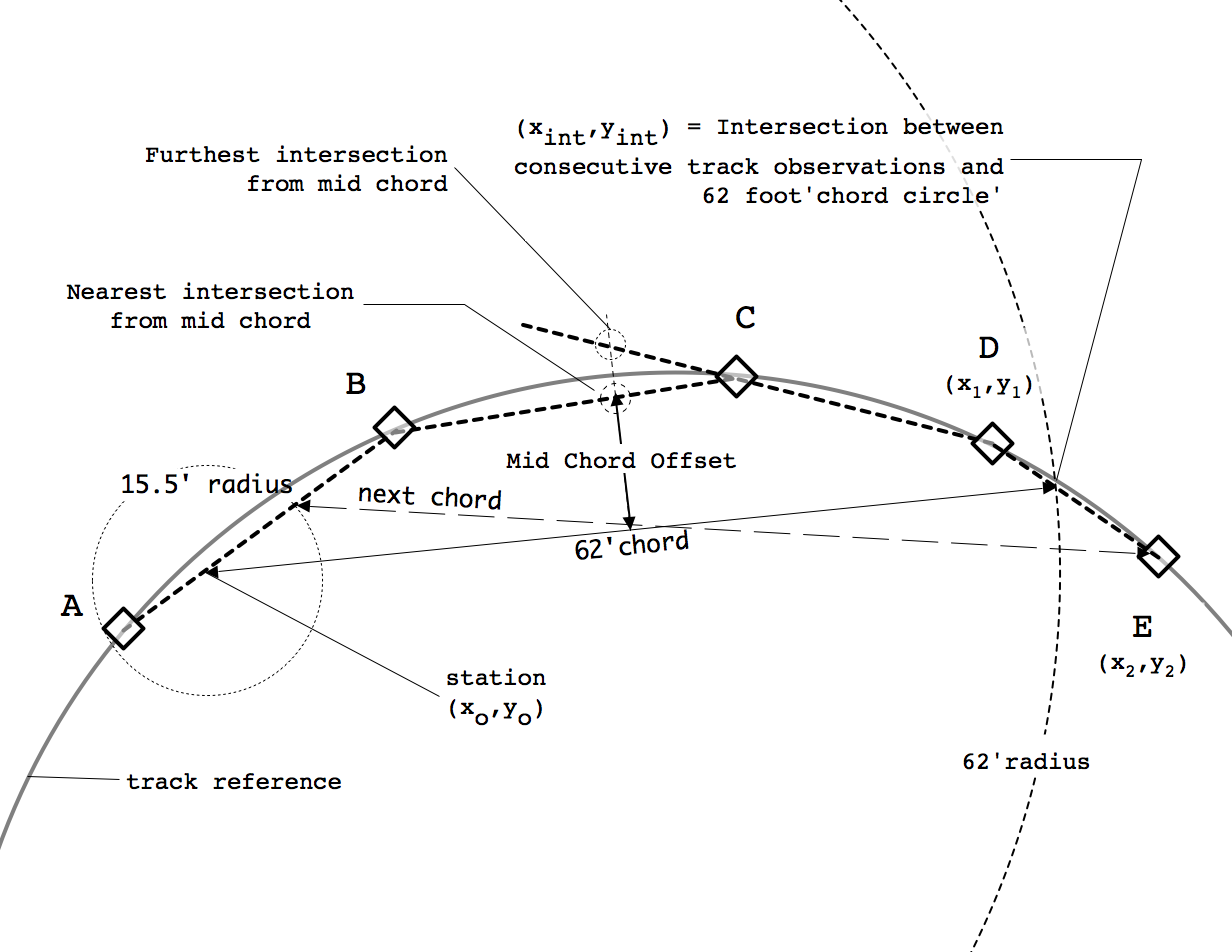
\includegraphics[width=13cm]{graphics/stringLining.png}
		\caption{Modeling the String Line Method from RTK Track Observations}
		\label{fig:strLine}
	\end{center}
\end{figure}

The MCO is determined from an line orthogonal with the mid point of the chord, and the mean of the intersection with the nearest and farthest of two lines projected from the three observations nearest to the middle ordinate (figure~\ref{fig:strLining} points B, C, and D). The distance from the chord mid point and the mean intersection determines the MCO. The degree of curve (chord definition) is then found from the MCO and chord length in feet by the relationship~\citep{1964hickerson}.
	\begin{equation}
		D_c = \frac{45840 \times MCO}{chord^2}
		\label{eqn:degOcrv}
	\end{equation}
	
The model assigns a mile post reference to $D_c$ using the location of the mean intersection and equation \ref{eq:accumSlopeD}.

The coordinates of the next station are found by intersecting the stationing distance in a similar fashion to the chord circle intersection. Figure~\ref{fig:strLining} illustrates determination of a 15.5 foot station. 

A railway can be described as a smooth, continuous shape. As an aid to exploring the $D_c$, a smoothing algorithm is applied to the $D_c$ verses mile post reference.  The \emph{rlowess}\footnote{The \emph{rlowess} method is a local regression using weighted linear least squares and a 1st degree polynomial model that assigns lower weight to outliers in the regression. The method assigns zero weight to data outside six mean absolute deviations~\citep{matlab09}.} method of the \emph{smooth} function in the Matlab \emph{Curve Fitting Toolbox}$^{TM}$ was selected as a data exploration tool.

RTK derived track alinements from multiple traverses were plotted and evaluated by:
\begin{itemize*}
	\item Determining descriptive statistics of a traverse over tangent track for both a specialized geometry car $D_c$ and a RTK equipmed Hi-Rail $D_c$. vs. mile post reference across identical tangent segments.
	\item Graphic correlation of $D_c$ across identical track segments for multiple traverses.
	\item Variability between degree of curve in selected tangent track segments modeled with RTK GNSS data against rail company provided track geometry vehicle data.
\end{itemize*}

Tangent segments were selected from the MP 209-207 GMRS data. The degree of curve variance was determined from the selected tangent segments.

% Track Occupancy Design
\subsection{Experiment Three: Determining Track Occupancy} 
This experiment asked whether a common track vehicle using RTK augmented GPS/GNSS was able determine track occupancy by obtaining position accuracy defined by the FRA for a location determination system. The FRA LDS requirement stated in \emph{Differential GPS: An Aid To Positive Train Control}~\citep{1995FRADiffe} page 6, establishes the criteria to\\
\begin{quotation}
``...determine which of two tracks a given train is occupying with a very high degree of assurance (an assurance that must be greater than 0.99999 or (0.9$_5$)). The minimum center-to-center spacing of parallel tracks is 11.5 feet...''\\
\end{quotation}
The FRA specification is interpreted here to mean an observation must have a cross-track error no greater than $\pm \frac{11.5}{2}$ feet within a confidence interval (1-${\alpha}$), where ${\alpha}$ = 0.00001 or 0.99999.

Several traverses of a parallel multitrack segment were made by RTK GNSS equipped Hi-Rail. A track segment was selected based on the length of the tangent or curve and existence of adjacent parallel track traverses. The first traverse was designated as a reference centerline, and the centerline coefficients for tangent track determined by regression using the Matlab function \emph{regress}.

In the tangent case, the Matlab function call took the general form: \emph{[b,bint,r,rint,stats] = regress (Northing, Easting, 1), ${\alpha}$}. 
The function output \emph{b} contained the coefficient estimates, \emph{bint} contains the upper and lower confidence bounds of the coefficient estimates, and \emph{r and rint} contain residuals and residual intervals that have no meaning in this analysis. The statistics contained in \emph{stats} contains ${R^2}$ statistic, the ${F}$ statistic and its p-value, and an estimate of the error variance.

The slope is converted to an azimuth and back bearing by the function \emph{slope2Az}, listed in Appendix B, page \pageref{software}. The azimuth of the tangent was verified using the graphical solution in the \emph{TGO} software.

The cross-track\footnote{Figure \ref{fig:trackRef} page \pageref{fig:trackRef}} distance between subsequent observations and the baseline was determined by the Matlab function \emph{perpDist2line}, listed in Appendix B, page \pageref{software}. The function determines the cross-track distance for all subsequent observations in the tangent segment using equation \ref{tanXtrack}.
%d = abs[(aX + bY +c)/srt(a^2 + b^2)]
\begin{equation}
d = \left|\frac{ax + by + c}{\sqrt{a^2 + b^2}}\right| \\
\label{tanXtrack}
\end{equation}
where a, b, c are the coefficients of the reference tangent, \emph{x} is the observation Easting and \emph{y} is the observation Northing.

For the circular curve case, the coefficients of the reference curve origin and radius are determined from Northing and Easting observation of the selected curve segment. The cross-track distance is determined by the difference between the circular curve radius and coordinate distance from the origin.

Circular curve coefficients were determined by the Matlab function \emph{regress}. The specific form

%crvAX = [crvA.easting*.2 crvA.northing*.2 numel(crv2.northing)*.-1]
%crvAY = [crvA.easting.^2 crvA.northing.^2]

% Tangent hypothesis test
The null hypothesis statement is the reference track is occupied if the distance between an RTK GNSS observation and the reference centerline is less than or equal to $\frac{11.5}{2}$ feet at a confidence of 100(1-${\alpha}$)\%. The Matlab function \emph{ztest}  was used for the z-test of the null hypothesis. The function output indicates whether the null hypothesis is a random sample from a normal distribution with mean distance ${\le}$ 5.75 feet and standard deviation $\sigma$, against the alternative that the mean is not ${\le}$ 5.75 feet. The result of the test is  indicates a rejection of the null hypothesis at the 100(1 - 0.00001)\% significance level.

\begin{equation}
	h_{0}: \mu_d \le \frac{11.5}{2}\\
\end{equation}
\begin{equation}
	h_{1}: \mu_d > \frac{11.5}{2}\\
\end{equation}

The null hypothesis asserts that the cross-track error population parameter is equal to or less than half the FRA centerline to centerline track spacing. Acceptance of the null hypothesis indicates statistical evidence exists to assert same track occupancy to the confidence interval specified by the FRA~\citep[pp. 6]{1995FRADiffe}.

Matlab command for regression statistics
input: y value, [x value, array of ones: numEl], alpha 
[b,bint,r,rint,stats] = regress(B.Northing,[B.Easting ones(numel(B.Easting),1)],0.00001)

The Matlab \emph{Statistics Toolbox} funtion \emph{ztest} performs a z-test of the null hypothesis that the cross-track error data is a random sample from a normal distribution with mean \emph{m} and standard deviation $\sigma$, against the alternative that the mean is not \emph{m}. The result of the test indicates a rejection of the null hypothesis at the (1-${\alpha}$) significance level.


Experiment three objectives sought to:
\begin{enumerate*}
	\item  Collect single epoch observations on a nominal 5 foot horizontal spacing with RTK augmented GPS on board a track vehicle over 29 continuous miles of mainline track.
	\item Determine the coefficients for the position of select tangent and circular track segments. Long tangent and circular segments will be selected to maximize the number of data.
	\item Determine the distance between subsequent observations by track vehicle to the reference tangent and curve segments.
	\item Determine if statistical evidence exists to indicate if RTK GNSS is capable of determining track occupancy of a vehicle meeting FRA performance standards for a location determination system.
\end{enumerate*}
% Variables
\emph{Variables of analysis}: The mobile instrument \#1 and \#2, table \ref{tab:inst} produced these variables:
\begin{itemize*}
	\item UTM, Zone 17 North, northing in US survey feet.
	\item UTM, Zone 17 North, easting in US survey feet.
	\item NAVD 88, height above ellipsoid, Geoid 2003, in US survey feet.
	\item Time (local, EST) and date of observation.
\end{itemize*}
% Instrumentation %
\section{Instrumentation}
Instruments used in the research are summarized in table \ref{tab:inst}.
% Table of instrumentation
\begin{center}
\begin{threeparttable}
	\caption{Instrumentation and Software}\label{tab:inst}
	\begin{tabular}{llll}%{ p{2.0cm} p{3cm} p{3cm} p{3cm}}
\toprule
	Designation & Instrument & Description &  Experiment\\
\midrule
	Ad hoc& Trimble 5700 & 24 ch. GPS receiver & 1\\
	Reference& Zephyr Geodetic & GPS antenna & \\
	Station& Trimmark III UHF radio & 450Mhz band, 25 watt& \\
\midrule
	CORS & NetRS/NetR5 & 24/72 ch. GPS\tnote{$\dagger$} /\-GNSS\tnote{$\ddagger$} & 2, 3\\
	& Trimble Zephyr Geodetic /2 & GPS/\-GNSS antenna &\\
	VRS & Trimble Network Infrastructure & Virtual Reference Station &\\
	& \emph{VRS} Net & version 2.83\tnote{$\dagger$} & 2, 3 \\
\midrule
	Static Module & Trimble R8 & 24 ch. GPS w/int. radio &1\\
	& Trimble TSC2 & Survey Controller &\\
\midrule
	Mobile\#1           & Trimble 5700 & 24 ch. GPS w/int. radio & 1\\
	& Trimble TSC2 & \emph{Survey Controller}v12.1x &\\
	& Trimble Zehyr & GPS antenna &\\
\midrule
	Mobile\#2                & Trimble R7 & 72 ch. GNSS receiver& 2, 3\\
	& Trimble TSC2       & \emph{Survey Controller}v12.1x &1, 2, 3\\
	& Trimble Zephyr 2 & GNSS antenna & 2, 3\\
\midrule
\multicolumn{3}{l}{Software}\\
	& National Geodetic Survey & Online User Positioning Service & 1 \\
	& Trimble \emph{Geomatic Office} & version 1.63 & 1, 2, 3 \\
	& Google Docs & Collaborative spreadsheet & 1\\
	& ESRI \emph{ArcMap}    & version 9.2     & 1 \\
	& Matlab 32-bit (maci)      &  version 7.8.0.347 (R2009a) & 1, 2, 3\\
	\bottomrule
	\end{tabular}
		\begin{tablenotes}
		\item[$\dagger$]{Owned and operated by the Ohio Department of Transportation, Aerial Mapping}
		\item[$\ddagger$]{Owned and operated by the N.J. Rahall Appalachian Transportation Institute}\\
		\end{tablenotes}
\end{threeparttable}
\end{center}

\begin{itemize*}
	\item An ad hoc reference station (AhRS) as listed in table \ref{tab:instruments} uses a stationary reference antenna to receive SV signals for manipulation by a GPS receiver to produce correctors for transmission over UHF data radio to a capable mobile GPS receiver.
	\item A single \emph{continuously operating reference station} (CORS) provides continuous data for RTK surveying applications.
	\item  A \emph{virtual reference station} (VRS) server provides differential positioning service across a large area from numerous CORS networked and synchronized with infrastructure software. Observations from each CORS in the network are pre-processed to generate models of the distance-dependent biases. Based on the model parameters and the user's approximate position, individual corrections can then be predicted, which enables differential positioning. The differential errors caused by ionospheric and tropospheric refraction, as well as satellite orbit errors are precisely estimated with networked RTK based on dual-frequency carrier phase observations regional network of CORS. Correction model parameters are determined to allow the prediction of the differential errors for the baseline between a master reference station and the user's position. Applying these corrections to code and carrier phase observations of the master reference station, VRS measurements are generated for RTK positioning of the rover receiver.
	\item A \emph{static survey} unit is an RTK enabled GPS or GNSS receiver used by a surveyor to determine the coordinate of a position by recording multiple-epoch observations while occupying the point of interest.
	\item A \emph{mobile survey unit} is an RTK enabled GPS orGNSS receiver used to determine the coordinates of a position while in motion by recording single epoch observations.
\end{itemize*}
			%%%%%%%%%%%%%%%%
			%  Data Validity and Integrity %
			%%%%%%%%%%%%%%%%
\section{Data Validity and Integrity}

% Validity
\emph{Validity}

Insuring the the validity of RTK GPS/GLONASS data relied on the quality control performed by the data collector software. A field notebook was kept to record various instrument and initial values (i.e., antenna height from top of rail, locomotive number, track points of interest) found during antenna alinement. The recorded values were programmed into the controller as a specific survey style to insure the use of identical calibration values between observation files during multi-day surveys and spanning months using a particular Hi-Rail.

The survey controller was programmed to reject observations that fell outside a threshold relative horizontal and vertical precision as determined by the receiver. A threshold value of 0.15 feet horizontal and 0.50 feet vertical was selected for the hump yard survey, and 0.10 feet horizontal and 0.20 feet vertical was selected for the alinement surveys. The threshold values were selected based on the manufacture's stated accuracy, the expected degradation due to reference station distance, the  receiver type, plus overhead. Receivers designated as GPS are capable of receiving and decoding only GPS SVs, while a GNSS receiver is capable of receiving GPS and GLONASS SVs. In all cases, the vertical threshold allowance is twice the horizontal value.

The hump yard observations were plotted using ESRI ArcMap software to produce color-mapped plan views of the yard. The color-mapped plot is similar to a contour map. However, where a contour map utilizes a triangulated irregular network to provide elevations over an area feature, the centerline top-of-rail line feature is of interest in a hump yard. Elevations were plotted as colored dots indicating an elevation range.

Color mapping relative vertical precision provides a graphical method of analysis for time-related SV reception quality. RTK GPS quality is dependent on satellite geometry, so serial observations of lower quality would be expected to appear together.

The track alinement model processes observations that are determined to be sequence by the software model. Changes in bearing between any two observations that approached 180$^{\circ}$ indicated the Hi-Rail reversed direction while recording of track observations. Points recorded in the reverse direction were not used.

% Integrity
\emph{Integrity}

During the hump yard experiment, several hundred points of interest\footnote{track switch points, retarder inlet and outlet, wheel detectors} (POI) were surveyed on the ground with the static survey instrument. The points were later translated such that the POI was relocated to the the track centerline.

Transferring the hump yard data to a CAD drawing used a web-based spreadsheet to enable  collaboration among the research team.

A check on point sequencing in the alinement model plots the sequence in three dimensions. The ordered sequence for each mile can be verified by examining the 3D plot.

% Summary
% Summary goes back to problem statement
\section{Summary}
The research method explores track measurement using commercial off-the-shelf RTK augmented GPS and GNSS instrumentation.  Each experiment examines the value of RTK augmentation to provide value in challenging railway measurements. The research examines the ability of single epoch RTK GNSS observations to act as a component of a location determination system.

Experiment 1 traversed an active hump yard with a locomotive equipped with RTK GPS instruments to observe track positions. The recorded positions were used to produce a profile for each track. The relative vertical precisions of the locomotive observations and reference station were analyzed for the influence of multipath reflections.

Experiment 2 traversed a continuous 29 mile segment of mainline track by a Hi-Rail equipped with RTK GNSS instruments. A model of the string line method was used to determine the ${D_c}$ for each mile, evaluate the model against rail company track charts for location, magnitude, and direction of curves. The model was used to 	evaluate the performance of RTK GNSS and the model against a specialized track geometry car over a comparable segment of tangent track.

Experiment 3 evaluated the ability to determine track occupancy by RTK GNSS. Five surveys traversed a parallel multitrack segment. The cross-track error between a baseline survey and subsequent surveys was evaluated in a tangent and circular curved segment. The statistical likelihood of estimating track occupancy meeting FRA guidelines for a location determination system was determined.


%% !TEX root = dissertation2.tex
\chapter{Results}

% Purpose
\section{Purpose}
The researcher sought to determine the viability of RTK GNSS augmentation to asses railway infrastructure and act as a reliable track vehicle locator capable of meeting the requirements of a location determination system as defined by the FRA by answering these questions:

1)\emph{Hump Yard Profile:}
Can a locomotive use RTK augmented GPS to measure the  vertical profile of bowl tracks in an automatic classification yard during production activities?

2)\emph{Horizontal Track Alinement:}
Can a common track vehicle use RTK augmented GPS/GNSS to determine the horizontal degree of curvature ($D_c$) comparable with specialized track geometry vehicles?

3)\emph{Track Occupancy:}
Can a common track vehicle use RTK augmented GPS/GNSS to meet the positioning requirements for track occupancy outlined by the FRA~\citep[pp.6-7]{1995FRADiffe} for a location determination system?

These experiments used common track vehicles equipped with survey-grade RTK GPS/GNSS instrumentation across yard and mainline track. The research examined three absolute positioning applications using RTK augmented GPS/GNSS in the context of a Class I railroad. The experiments addressed these questions:

1. \emph{Hump Yard Profile}\\
%Relative precision - Precision is defined as a measure of the tendency of a set of numbers to cluster about a number determined by the set (e.g. the mean). The usual measure is the standard deviation with respect to the mean. Relative precision denotes the tendency for the various components (X, Y, Z) between one station and other stations in the network to be clustered about the adjusted values. Current custom is to express relative precision at the two-standard deviation (95% confidence) level. This may be stated in terms of a relative error ellipse or as a proportion of the separation distance (e.g. 10 ppm or 1:100,000). 
Can a locomotive equipped with RTK GPS instrumentation be used to measure the  vertical profile of bowl tracks in an automatic classification yard during humping operations?
The question was answered through the completion of several objectives:
\begin{itemize}
\item A method was developed for measuring track profiles in the bowl area of an active hump yard.
\item The method was demonstrated by use of an ad hoc GPS reference station transmitting correctors to a RTK GPS receiver aboard a yard locomotive. 
\item A relative vertical precision distribution was determined from the RTK GPS observations.
\item Track profiles were developed from the locomotive survey data.
\end{itemize}

2. \emph{Horizontal Track Alinement}\\
Can a common track vehicle use RTK augmented GPS/GNSS observations to determine the horizontal degree of curvature over tangent track comparable with specialized track geometry vehicles?
The question was answered through the completion of several objectives:
\begin{itemize}
\item A method was developed for measuring track horizontal position from a track inspector's Hi-Rail vehicle.
\item A software model was developed to determine the degree of curvature using the string lining method.
\item A parameter estimation of the ${D_c}$ variability of the model and a track geometry car was determined for selected tangent track segments.
\end{itemize}

3. \emph{Track Occupancy}\\
Can a common track vehicle using RTK augmented GPS/GNSS instrumentation meet the positioning requirements for track occupancy outlined by the FRA for a location determination system?
The question was answered through the completion of several objectives:
\begin{itemize}
\item An analytical method was developed to determine the variance in a series of RTK GNSS measured track positions from specific geometric segments.
\item A hypothesis test was used to determine the likelihood of RTK GNSS position measurements to meet the FRA criteria for reliable track occupancy.
\end{itemize}

\section{Hump Yard Profile Results}
The objective of experiment one was to use a locomotive to survey an active hump yard to produce track profiles from RTK augmented track observations. A hump yard owned by CSXT and located in Hamlet North Carolina was the subject of this experiment. Track centerline top-of-rail observations recorded from locomotive and ground observations are summarized in \ref{tab:humpData}. The human effort expended during the yard survey is presented in table \ref{tab:labor}.
% Table of human resource usage
\begin{center}
\begin{table}[!ht]
\caption{Hump Yard Survey Human Resource Utilization}\label{tab:labor}
\begin{tabular}{llll}%{ p{4cm} p{3cm} p{4cm}}
\toprule
Classification & Labor Hours & Task Description\\
\midrule
Surveyor, locomotive & 5 shifts of 8 hours & manage locomotive GPS  & \\
Locomotive operator & 5 shifts of 8 hours & manage locomotive, switches & \\
Surveyor, ground & 2 sessions of 3 hours & collect POI, set bench marks & \\
Watchmen lookout & 2 sessions of 3 hours & safety lookout for ground surveyor\\
Company escort & 5 hours & safety briefings, guide\\
\bottomrule
Total hours & 97 hours &\\
\end{tabular}
\end{table}
\end{center}
%An analysis of the vertical precision of the observations will be used to determine if statistical evidence is present to indicate the one sigma mean vertical precision of RTK augmented GPS observations by locomotive in a hump yard is 0.1 feet or less.
The resulting OPUS reports generated from the two reference station observation sessions referred to in chapter 3, page \pageref{baseRefPeriod} are exhibited in Appendix A, pages \pageref{opus1}~-~\pageref{opus2}.

Adjustments to the autonomous GPS position of the ad hoc reference station (CP1) used during the survey are listed in table \ref{tab:AdHocPos}. An error of 0.003 feet was introduced in the elevation adjustment of CP1. The likely cause was in transcribing the calculated elevation adjustment into the TGO software. Consequently, the transcription error was propagated to each observation during recomputing point positions from the base station to observation vectors. The error was not significant to the work, as it was less that half the manufacturer's stated $\pm$~0.066 foot vertical accuracy of the GPS total station.

 % Table of reference station corrections
\vspace{-30pts}
\begin{center}
\begin{threeparttable}
	\caption{Reference Station Adjustment}
	\label{tab:AdHocPos}
	\begin{tabular}{l c c c}
	\toprule
	Point & Northing & Easting & Elevation\\
	\midrule
	CP1 autonomous & 426094.534 & 1802674.100 & 462.354 \\
	OPUS 89691472 & 426095.398 & 1802677.668 & 464.944  \\
	OPUS 89691491 & 426095.376 & 1802677.685 & 465.107  \\
	mean OPUS & 426095.387 & 1802677.677 & 465.026 \\
	\midrule
	EB1559 publlished& 422425.72 & 1795001.00 & 389.54 \\
	CP1 to EB1559 vector & $\Delta$-3721.022 & $\Delta$-7653.073 & $\Delta$-77.070 \\
	\midrule
	CP1 adjusted & 426095.387 & 1802677.677 & 465.081\tnote{} \\
	\midrule
	residuals&&&\\
	$\Delta$ OPUS & 0.000 & 0.000 & +0.055\\
	$\Delta$ EB1559 & +0.068 & -0.045 & +0.003\\
	\bottomrule
	\end{tabular}
%	\begin{tablenotes}
%		\item[\dag]{Elevation adjusted to EB1559.}
%	\end{tablenotes}
\end{threeparttable}
	\end{center}

Two TEQC reports were generated from the two reference station observing sessions. The reports detail the quality of observations by the reference station during the periods referenced in chapter three page \pageref{baseRefPeriod} referenced in Appendix A, pages \pageref{teqc1} and \pageref{teqc2}. The overview graphically depicts the GPS SVs visible during the base station observation period. Additional information in the reports the quality of reference station observations.

% Table of Hump Yard Results
\begin{table}[ht]
	\begin{center}
	\caption{Relative Vertical Precision Summary}
	\label{tab:humpData}
	\begin{tabular}{c c c c c c}
	\toprule
	$\alpha$ = 0.01&&&conf.int.&&conf.int.\\
	Tracks & N & $\mu$ &$\mu$& $\sigma$&$\sigma$\\
	\midrule
	58 & 9,570 & 0.07753 & 0.07640 to 0.07866 & 0.0429 & 0.04213 to 0.04373\\
	\bottomrule
	\end{tabular}
	\end{center}
\end{table}

% Shot list

% Spreadsheets
Spreadsheets were constructed in Google Docs, and shared among the research team. A workbook was created for each track group, and individual worksheets constructed for each track. Algorithms for determining horizontal linear reference and elevation scaling are available. A hyperlink to each group workbook is exhibited in Appendix A, page .

% Profile drawings
Track profiles were plotted with a drawing provided by CSX as the result of a January 2001 survey by others. Attempts at recovering the 2001 benchmarks were unsuccessful.

The horizontal axis of each drawing represented the horizontal linear track reference and the vertical axis representing the elevation. A reference mark on the drawing was matched with the track structure observed during the survey. Linear references from the drawing were assigned to the match mark in the spreadsheet, and the linear reference of each track observation was determined by horizontal stationing equation \ref{eq:horzSta} . 

Elevations were plotted twice, first in a 1:1 scale with the design yard grade, and secondly exaggerated 5:1 to better discern profile differences. Entries in table \ref{tab:profiles} Appendix A, page \pageref{profiles} are hyperlinks to D size drawings (.pdf format). 

% Relative vertical precision
The relative vertical precision of each point observed calculated by mobile\#1 was recorded. The descriptive statistics for the relative vertical precision is listed in table \ref{tab:humpData}.

Appendix A figure \ref{vert_hist} presents a histogram of the vertical precisions in addition to descriptive statistics for the aggregate observations.

\emph{Hump Yard Profile Summary}

An RTK survey of the Hamlet Terminal by locomotive was completed in five, eight hour shifts. The first day was consumed by yard safety, yard facility familiarization, and antenna alignment. Four eight hour shifts were sufficient to complete a traverse of every open track in the bowl. The survey strategy first traversed the pullout end to the foul point. The pull-out end humpmaster preplanned and coordinated runs through alley\footnote{A clear track.} track with the locomotive engineer, though the survey locomotive was also sporadically used to pull cars during the survey.

The hump end was surveyed during the last day's shift change. During shift change, the pin puller and other hump end personnel undergo a transition period of exchanging relevant yard information, with the oncoming shift receiving a current safety briefing. The hump-end yard master took advantage of the staggered shift change to switch the survey locomotive through each hump and group lead track on the hump end. The brief period between shift changes did not allow time for individual group lead and tracks to be renamed in the survey controller. Consequently the data was separated manually during post-survey office work.

Post survey work consisted of adjustment to the reference station position; recalculating point positions from station to point vectors; deconstructing the aggregated points by track and lead; separating points into layers based on track and lead; adjusting ground points so as to be coincident with the centerline; renaming point sequences and exporting each sequence to a spreadsheet; applying a linear reference to each point; scaling the elevations in preparation to plot on an existing CAD drawing; plotting and printing the CAD generated profiles.

\section{Determining Alinement by Hi-Rail Results}
%Experiment 2 Analysis

Mainline track was surveyed by table \ref{tab:instruments} mobile\#2, mounted to a track inspector's Hi-Rail, over mainline track listed in table \ref{tab:Hi-RailSurvey}.

Continuous data recording during the 20 January 2010 survey was impeded by unexpected receiver operation. The receiver was unable to initialize with a new VRS without cycling receiver power after each VRS update. The problem lead to numerous unexpected data gaps during the traverse. The problem was identified and corrected by updating the receiver firmware. The receiver performed as expected during subsequent surveys. Mainline surveys traversing the Kanawaha Subdivision from mile post (MP) 494 to 523 are summarized in table \ref{tab:Hi-RailSurvey}.

% Mainline Survey Inventory
\begin{table}[ht!]
	\begin{center}
	\caption{RTK Surveys By Hi-Rail}
	\label{tab:Hi-RailSurvey}
		\begin{tabular}{c c c c c l}
			\toprule
			Ref.&Date& Traverse&Track(s)&CL Observations&Note\\
			\midrule
	A & 20 January 2010   &MP494 to 523 & 1,2           & 18,095 &f/w 1.02\\
	B & 5 February 2010   &MP495 to 512 & 2,1,2        & 15,225 &f/w1.13, traffic \\
	C & 14 February 2010 &MP495 to 523 & 1, 2          & 22,866 &f/w1.13\\
	D & 3 March 2010       &MP495 to 522 & 2,3,2        & 19,993 &f/w1.13\\
	E & 18March 2010      &MP494 to 523  & 1             & 21,001 &f/w1.13\\
			\bottomrule
	\end{tabular}
	\end{center}
\end{table}

Output generated from processing RTK observations with string line model are cataloged in Appendix B. The rail company provided track chart precedes each segment between MP494 and 523 traversed by a RTK equipped HI-Rail. Correlation between model output and charted features is produced in table \ref{tab:Hi-RailTraverse}. 

Two discrepancies between the track chart values and model output were discovered.
\begin{itemize}

\item The track charts indicates the curve beginning at MP {508.9} is a curve to the right (referenced to the direction of travel, increasing mile post). The model determined the a curve was to the left. The model determined value is verified by examination of a plan view of the track observations between MP 508 and 509, figure \ref{crv508_9}.
\begin{figure}[!ht]
	\begin{center}
	\vspace{0pt}
	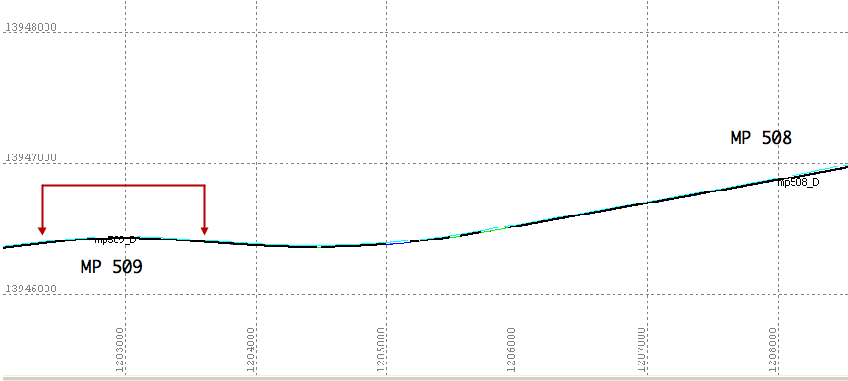
\includegraphics[scale=0.30]{graphics/508_9curve}
	\caption{Plan View MP 508-509}
	\label{crv508_9}
	\end{center}
	\vspace{-10pt}
\end{figure}

\item The track chart indicates the 1 degree curve to the right at mile post 521.15 extends approximately 0.15 miles. The model determined the curve extends from MP 521.15 to 521.83, or one half mile longer than indicated on the track chart. The model determined value is verified by examination of a plan view of the track observations between MP 521 and 522, as illustrated by figure \ref{crv521}.

\begin{figure}[!ht]
	\begin{center}
	\vspace{0pt}
	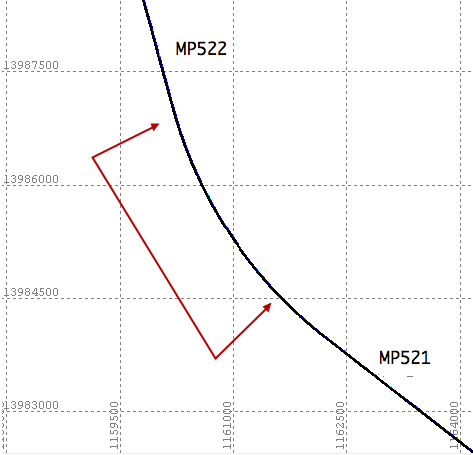
\includegraphics[scale=0.30]{graphics/521-522curve}
	\caption{Plan View MP 521-522}
	\label{crv521}
	\end{center}
	\vspace{-10pt}
\end{figure}

\end{itemize}

Features causing loss of GNSS signal (LOS) were documented by referencing the location to the track chart. When not evident from the track chart, the geodetic coordinates of a point before LOS was entered into Google Maps, and the aerial image examined. This method was effective in determining the location of signal bridges and several overpasses.

Table \ref{tab:Hi-RailTraverse} also references rail company track chart (TC) values for ${D_c}$ and mile length for comparison with the model output. Track charts do not provide exact values for individual tracks, therefore the comparison serves only to verify the quantity and magnitude of alinement features.

\begin{center}
% Setup for longtable
\begin{longtable}{c l c l}
\caption[RTK Hi-Rail Traverse MP 494-523, Alinement Annotation]{RTK Hi-Rail Traverse MP 494-523, Alinement Annotation}
\label{tab:Hi-RailTraverse} \\
%This is the header for the first page of the table...
\hline
   \multicolumn{1}{c}{\textbf{MP Reference}} &
   \multicolumn{1}{l}{\textbf{Feature}} &
   \multicolumn{1}{c}{\textbf{TC Value}} &
   \multicolumn{1}{l}{\textbf{Note}} \\
\hline
\endfirsthead

%This is the header for the remaining page(s) of the table...
\multicolumn{4}{c}{{\tablename} \thetable{} -- Continued} \\[0.5ex]
\hline
   \multicolumn{1}{c}{\textbf{MP Reference}} &
   \multicolumn{1}{l}{\textbf{Feature}} &
   \multicolumn{1}{c}{\textbf{TC Value}} &
   \multicolumn{1}{l}{\textbf{Note}} \\
\hline
%  \\[-1.8ex]
\endhead

%This is the footer for all pages except the last page of the table...
\midrule
\multicolumn{4}{r}{{Continued next page\ldots}} \\
\endfoot

%This is the footer for the last page of the table...
\bottomrule
\endlastfoot
494-495 & mile length & 8,858' &  Hi-Rail:8,949' \\
	494.05&curve&$3^{\circ}$03'R&\\
	494.46&curve&$2^{\circ}$45'L&\\
	494.65&curve&$2^{\circ}$30'R&\\
495-496 & mile length & 5,295' &  Hi-Rail:5,414' \\
	495.05&curve&$2^{\circ}$30'R&\\
	495.46&curve&$2^{\circ}$30'L&\\
	495.6-495.7&I-64 overpass&&LOS\\
\hline
496-497 & mile length & 5,255' &  Hi-Rail: 5,323' \\	
	496.05&curve&$3^{\circ}$45'L&\\
	496.25&curve&$1^{\circ}$00'L&\\
497-498 & mile length & 5,276' &  Hi-Rail: 5,340' \\
	497.3&curve&$0^{\circ}$45'L&\\
	497.61& & & LOS, VRS update\\
498-499 & mile length & 5,290' &  Hi-Rail: 5,342' \\
	498.6&curve&$2^{\circ}$00'R&\\
499-500 & mile length & 5,283' &  Hi-Rail: 5,342' \\
500-501 & mile length & 5,280' &  Hi-Rail: 5,356' \\
	500.4&curve&$2^{\circ}$32'R&\\
\hline
	501.03-501.12&cross over&&cross over, track 1 to 1\\
	501.15-501.35&Guyandotte River Bridge&&LOS\\
	501.35&curve&$4^{\circ}$14'L&\\
	501.6-501.67&29th Street overpass&&LOS\\
	501.9&curve&$1^{\circ}$33'L&\\
	501.95&curve&$1^{\circ}$33'R&\\
501-502 & mile length & 5,266' &  Hi-Rail: 5,316' \\
	502.62-502.69&cross over&&track 2 to 1\\
502-503 & mile length & 5,383' &  Hi-Rail: 5,208' \\
	503.4&curve&$1^{\circ}$15'L&\\
	503.55&curve&$1^{\circ}$33'R&\\
504-505 & mile length & 5,196' &  Hi-Rail: 5,281' \\
	504.05&curve&$2^{\circ}$56'R&\\
	504.15&curve&$4^{\circ}$30'L&\\
	504.52&curve&$0^{\circ}$55'R&\\
	504.6&curve&$1^{\circ}$05'L&\\
	504.85&curve&$2^{\circ}$00'L&\\
	504.92-504.96&signal bridge&&LOS\\
505-506 & mile length & 5,286' &  Hi-Rail: 5,335' \\
	505.0&spiral&from $2^{\circ}$00'L&\\
	505.5&curve&$1^{\circ}$00'R&LOS@505.55\\
\hline
506-507 & mile length & 5,189' &  Hi-Rail: 5,256' \\
	506.24&curve&$0^{\circ}$32'L&\\
	506.34-506.41&17th Street interchange&&LOS\\
	506.7-507.78&signal bridge&&LOS\\
	506.78&curve&$1^{\circ}$55'R&\\
507-508 & mile length & 5,255' &  Hi-Rail: 5,327' \\
	507.95&curve&$0^{\circ}$23'R&\\
508-509 & mile length & 5,262' &  Hi-Rail: 5,337' \\
	508.37-508.57&Spring Valley Road overpass&&LOS\\
	508.57&curve&$0^{\circ}$45'R&\\
	508.65&signal bridge&& LOS \\
	508.9&curve&$1^{\circ}$18'R&TC error, left\\
509-510 & mile length & 5,280' &  Hi-Rail: 5,355' \\
	509.0&spiral&$1^{\circ}$18'R  & TC in error, left\\
	509.21&curve&$0^{\circ}$18'L&\\
	509.56&curve&$0^{\circ}$28'L&\\
510-511 & mile length & 5,280' &  Hi-Rail: 5,336' \\
	510.2&curve&$1^{\circ}$05'R&\\
	510.7&curve&$3^{\circ}$23'R&\\
	510.95&signal bridge& &LOS\\
\hline
511-512 & mile length & 5,231' &  Hi-Rail: 5,319' \\
	511.72-511.8&Norfolk Southern overpass&&LOS\\
512-513 & mile length & 5,249' &  Hi-Rail: 5,349' \\
	512.52-513&Big Sandy River Bridge&&LOS\\
513-514 & mile length & 5,264' &  Hi-Rail: 5,408' \\
	513.0&curve&$4^{\circ}$51'R&\\
	513.31&signal bridge& &multipath\\
	513.6&curve&$6^{\circ}$23'L&\\
	513.7&curve&$3^{\circ}$00'R&\\
	513.92&curve&$3^{\circ}$00'L&\\
514-515 & mile length & 5,263' &  Hi-Rail: 5,293' \\
	514.0   &curve&$3^{\circ}$00'L& \\
	514.2   &curve&$2^{\circ}$00'R& \\
	514.8   &curve&$2^{\circ}$00'L& \\
	514.55 &signal bridge& &LOS\\
515-516 & mile length & 5,240' &  Hi-Rail: 5,318' \\
	515.0 &curve&$0^{\circ}$45'L& \\
	515.2 &curve&$1^{\circ}$30'R& \\ 
	515.5 &curve&$1^{\circ}$15'R& \\
	515.6 &signal bridge& &LOS\\
	515.8 &curve&$0^{\circ}$45'L& \\
\hline
516-517 & mile length & 5,047' &  Hi-Rail: 5,110' \\	
	516.12&curve&$3^{\circ}$00'R&\\
	516.78-517&curve&$1^{\circ}$00'L&LOS\\
517-518 & mile length & 5,432' &  Hi-Rail: 5,530' \\
	517.0&curve&$1^{\circ}$00'L & to $3^{\circ}$00'L\\
	517.43&curve&$1^{\circ}$30'L&\\
	517.6&curve&$4^{\circ}$15'L&\\
518-519 & mile length & 5,733' &  Hi-Rail: 5,821' \\
	518.05&curve&$1^{\circ}$00'R&\\
	518.23&curve&$1^{\circ}$15'L&\\
	518.4&curve&$0^{\circ}$00'&<sic>\\
	518.41&signal bridge& &multipath\\
	518.5&curve&$0^{\circ}$45'R&\\
519-520 & mile length & 4973' &  Hi-Rail: 5,059' \\
	519.1&curve&$1^{\circ}$30'L&\\
	519.15-519.34&2 signal bridges & &LOS\\
	519.2&curve&$1^{\circ}$00'R&\\
	519.6&curve&$2^{\circ}$00'L&\\
	519.65&curve&$2^{\circ}$00'R&\\
	519.8&curve&$2^{\circ}$30'L&\\
	519.9&curve&$1^{\circ}$45'R&\\
520-521 & mile length & 5,322' &  Hi-Rail: 5,431' \\
	520.5&curve&$2^{\circ}$15'R&\\
	520.55-520.69&Armco overpass& &LOS\\
\hline
521-522 & mile length & 4,972' &  Hi-Rail: 5,357.6' \\
	521.12-521.82&curve&$1^{\circ}$00'R&TC curve length error\\
522-523 & mile length & 5,023' &  Hi-Rail: 5,099' \\
	522.1-522.25&AK Steel Entrance Rd&&LOS\\
	522.6&curve&$1^{\circ}$00'L&\\
	522.9&curve&$0^{\circ}$30'L&\\
\end{longtable}
\end{center}
\vspace{-30pt}

% Measure method comparison between GMRS and Hi-Rail
To answer the research question asking if the RTK Hi-Rail method of determining $D_c$  was comparable with specialized inspection vehicles, measurements obtained from CSX for a GMRS inspection vehicle were compared with the output from the string line model using observations from a RTK GNSS equipped Hi-Rail. The two methods traversed CSX C\&O Ohio Subdivision between mile post 211 and 207. Illustration \ref{gmrs_HiRail} provides a graphic solution to the smoothed $D_c$ vs. mile post values obtained from both methods across the segment.

\begin{center}
\begin{longtable}{c c c c}
\caption[GMRS \& RTK Hi-Rail Comparision, MP 211-207, Alinement Annotation]{GMRS \& RTK Hi-Rail Comparision, MP 211-207, Alinement Annotation}
\label{tab:gmre_Hi-RailTrav} \\
%This is the header for the first page of the table...
\hline
   \multicolumn{1}{c}{\textbf{MP Reference}} &
   \multicolumn{1}{c}{\textbf{Feature}} &
   \multicolumn{1}{c}{\textbf{TC Value}} &
   \multicolumn{1}{c}{\textbf{Note}} \\
\hline
\endfirsthead

%This is the header for the remaining page(s) of the table...
\multicolumn{4}{c}{{\tablename} \thetable{} -- Continued} \\[0.5ex]
   \multicolumn{1}{c}{\textbf{MP Reference}} &
   \multicolumn{1}{c}{\textbf{Feature}} &
   \multicolumn{1}{c}{\textbf{TC Value}} &
   \multicolumn{1}{c}{\textbf{Note}} \\
\hline
%  \\[-1.8ex]
\endhead

%This is the footer for all pages except the last page of the table...
\midrule
\multicolumn{4}{r}{{Continued next page\ldots}} \\
\endfoot

%This is the footer for the last page of the table...
\bottomrule
\endlastfoot
	211-210 & mile length & 5,328' & GMRS:5,018' Hi-Rail:5,368' \\
	210.7     & curve &$2^{\circ}$15'L &\\
	210-209 & mile length & 5,263' & GMRS:4,973' Hi-Rail:5,314' \\
	209.6     & curve &$1^{\circ}$15'L &\\
	209.15   & curve &$1^{\circ}$00'L &\\
	209-208 & mile length & 5,252' & GMRS:5,027' Hi-Rail:5,318' \\
	208.8     & curve &$3^{\circ}$15'R &\\
	208.45   & curve &$1^{\circ}$15'L &\\ 
	208.0     & curve &$3^{\circ}$00'R &\\ 
	208-207 & mile length & 5,678' & GMRS:5,384' Hi-Rail:5,586' \\
	207.5     & curve &$5^{\circ}$00'R &\\ 
\end{longtable}
\end{center}

The longest tangent portion of the segment under study extends from MP 210.4 to 209.75, and was selected to determine the $D_c$ variance for the GMRS and the Hi-Rail RTK methods. An ideal measurement over an ideal tangent would result in an instantaneous $D_c$ value of zero at each point of measurement. The 201.4-209.75 tangent segment was assumed ideal. The variation from zero $D_c$ was determined for each method. Table \ref{tab:tanComp} provides descriptive statistics for $D_c$ values derived from each method. 

\begin{figure}[htpb]
	\begin{center}
	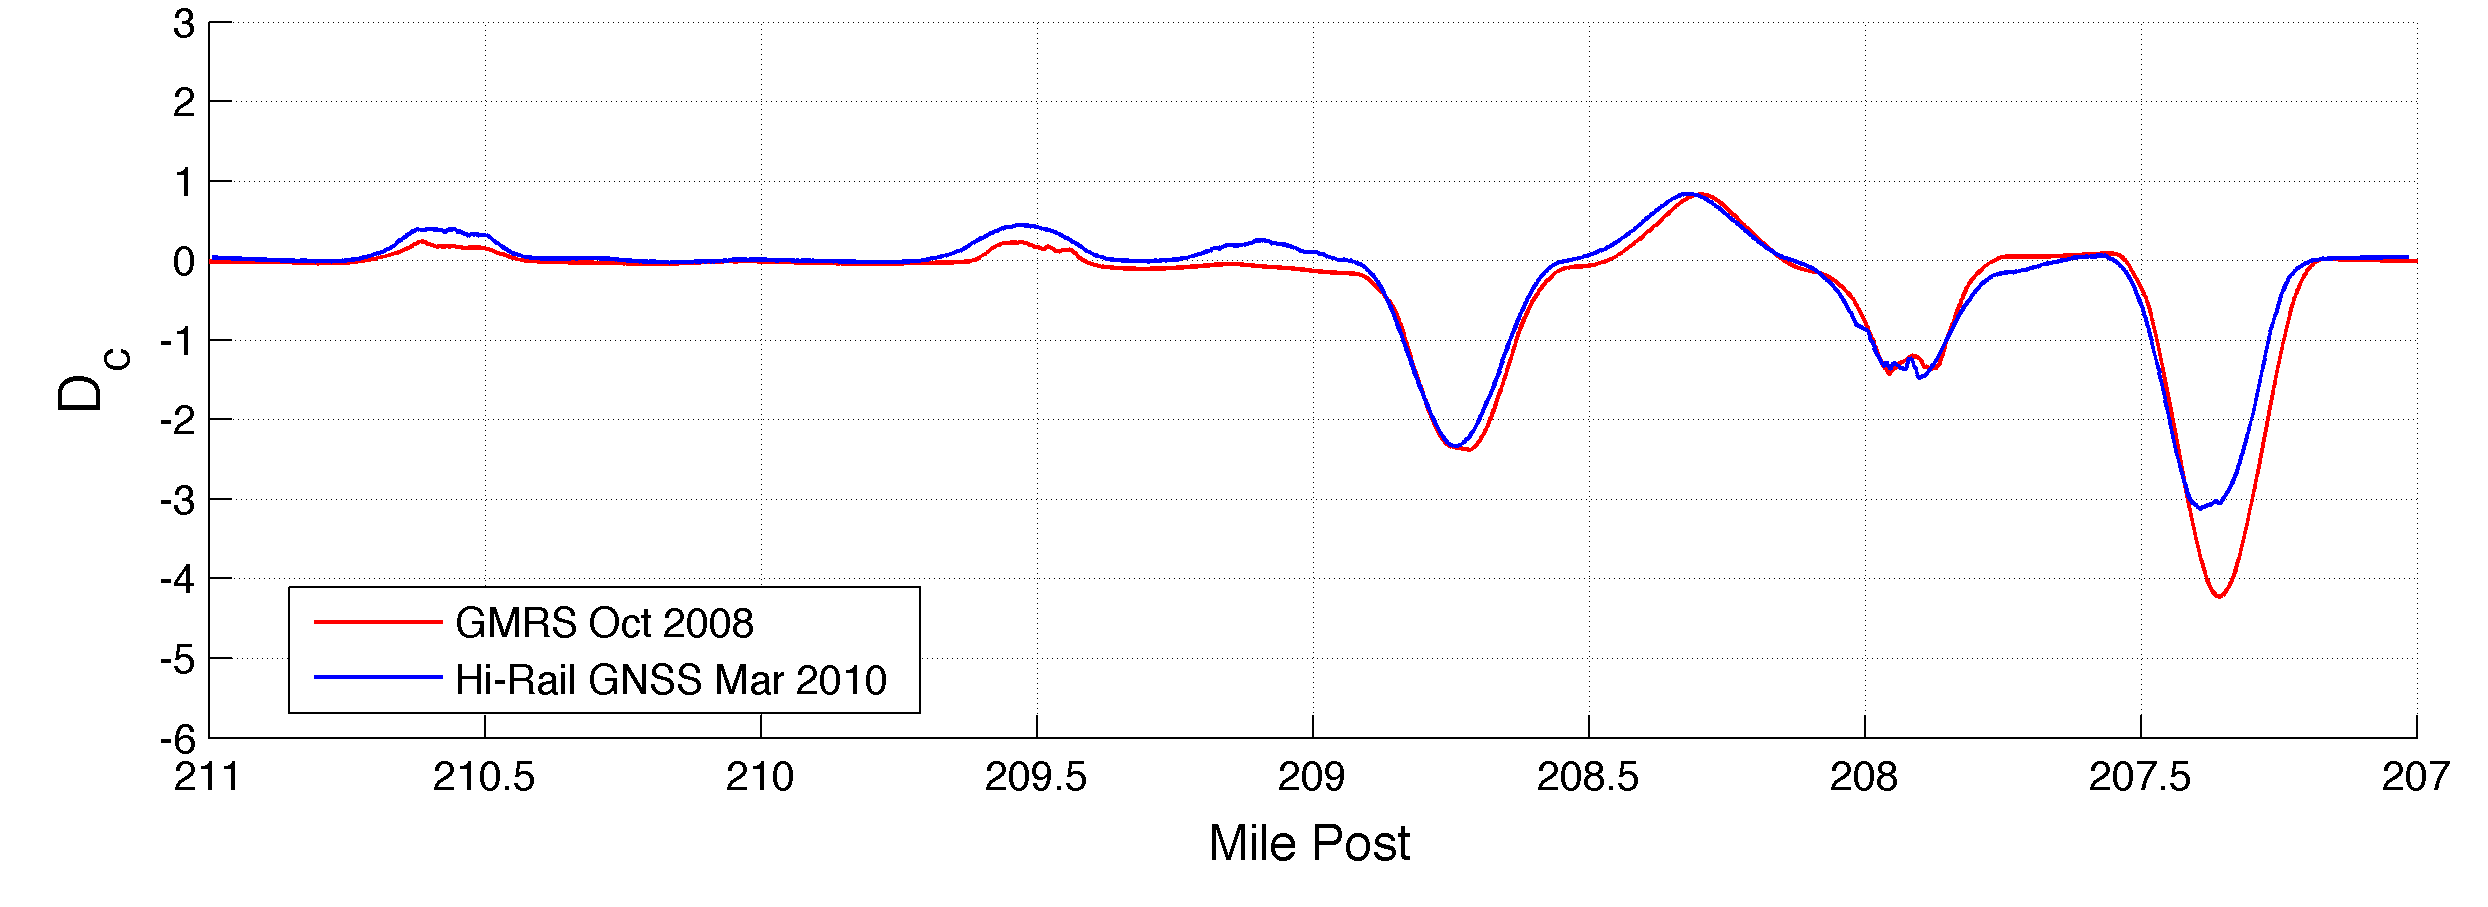
\includegraphics[scale=0.60]{graphics/GMRS_HiRail}
	\caption{GMRS and RTK GNSS Hi-Rail Comparison}
	\label{gmrs_Hi-Rail}
	\end{center}
\end{figure}

\begin{table}
\begin{center}
\caption{GMRS and RTK GNSS Hi-Rail Comparison, MP210.4-209.75 tangent}
\label{tab:tanComp}
\begin{tabular}{c c c c c c c}
\toprule
Vehicle&Stationing&N&${\mu}_{D_c}$&95\% CI&${\sigma}_{D_c}$&95\% CI\\
\midrule
GMRS&1 ft     &3,253&-0.02637&  -0.0307  -0.0219&0.1306&   0.1275   0.1339\\
Hi-Rail&15.5 ft&222   &-0.00417&-0.04106  0.03271&0.2789&0.2551   0.3076\\
\bottomrule
\end{tabular}
\end{center}
\end{table}

A histogram approximates the probability destiny function of the ${D_c}$ values. GMRS measurement deviation from zero is illustrated in figure \ref{gmrs_hist}. RTK GNSS Hi-Rail deviation illustrated in figure \ref{Hi-Rail_hist}. Both systems indicate a normal error distribution around zero ${D_c}$.

\begin{figure}[htpb]
	\begin{center}
	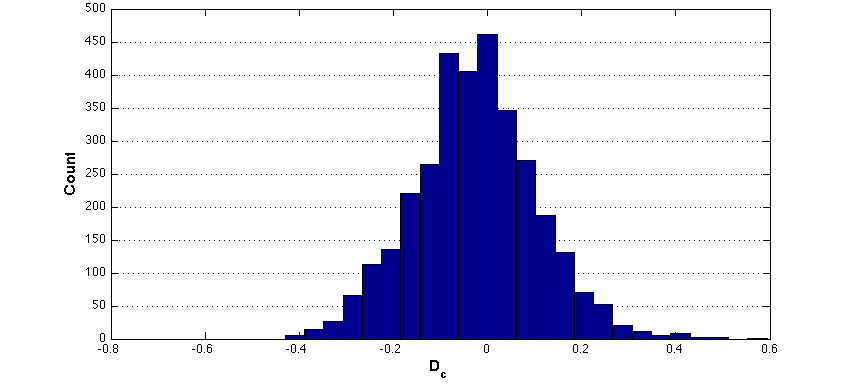
\includegraphics[scale=0.5]{graphics/GMRS_tanHist}
	\caption{GMRS ${D_c}$ Histogram, 210.4 to 209.75 tangent}
	\label{gmrs_hist}
	\end{center}
\end{figure}
\vspace{-40pt}
\begin{figure}[htpb]
	\begin{center}
	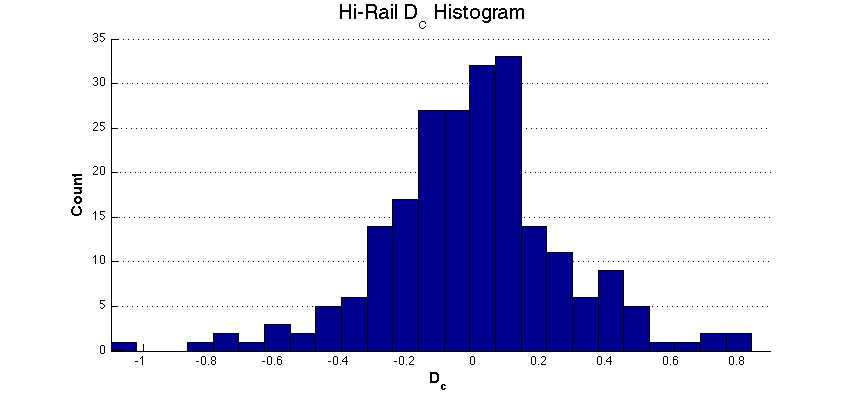
\includegraphics[scale=0.50]{graphics/HiRail_tanHist}
	\caption{Hi-Rail ${D_c}$ Histogram, 210.4 to 209.75 tangent}
	\label{Hi-Rail_hist}
	\end{center}
\end{figure}

%Track Occupancy Results
\section{Track Occupancy Results}
The question answered by experiment 3 was whether statistical evidence exists to determine if RTK GNSS as the sole position measurement instrument can meet the positioning requirements for track occupancy outlined by the FRA for a location determination system (LDS).

The question was answered through the completion of several objectives:
\begin{itemize}
\item An analytical method was developed to determine the variance in a series of RTK GNSS measured track positions from specific geometric segments surveyed by a common track vehicle.
\item A hypothesis test determined the likelihood of RTK GNSS position measurements in tangents and circular curves to meet the FRA criteria for reliable track occupancy.
\end{itemize}

The hypothesis test determines if sufficient statistical evidence exists to determine if RTK GNSS measurements conform to the criteria set by the FRA to enable the ability to distinguish what track a train in on in multi-track parallel segments.

Table \ref{tab:tanRegress} presents the result of a simple linear least squares regression performed on (Easting,Northing) coordinate pairs between mile post reference 498.9 and 500.2 for each of five surveys. Track position observations traversing three parallel tangent track of the same approximate length were recorded during five separate surveys. The correlation statistic ${R^2}$ for each regression was 0.99998 or better. The worse case variance around the centerline was exhibited on track 3. The regression excursive characterizes the observations of five surveys performed over a three month period for a section of tangent track over a mile in length.

\begin{table}[!htpb]
	\begin{center}
	\caption{Tangent Regression Coefficients, MP 498.9 to 500.2}
	\label{tab:tanRegress}
		\begin{tabular}{c c c c c c c}
\toprule
%\multicolumn{3}{l}{$\alpha = 0.00001$}\\
	Survey & Track & N  & Slope  & Y Intercept & Variance & Azimuth$^{\circ}$\\
\midrule
	A & 2 & 1,189 & 0.10220168 & 13825809.25 & 0.02259 & 264.164536\\
	B & 2 & 1,244 & 0.10219667 & 13825815.49 & 0.02208 & 264.164821\\
	C & 3 & 1,152 & 0.10208429 & 13825969.10 & 0.05664 & 264.171193\\
	D & 1 & 1,158 & 0.10213959 & 13825873.25 & 0.02432 & 264.168057\\
	E & 3 & 1,156 & 0.10209947 & 13825950.11 & 0.05338 & 264.170332\\
	\bottomrule
	\end{tabular}
	\end{center}
\end{table}

The cross-track error was determined between each point surveyed between mile post reference 498.9 and 500.2 and a centerline described from the regression coefficients of the tangent of survey A, presented in table \ref{tab:tanRegress}.
% Hypothesis test
\needspace{3\baselineskip}

Table \ref{tab:tanHypo} provides the result of the hypothesis test for each survey between M 498.9 and 500.2.

\begin{table}[htpb]
	\begin{center}
	\caption{Tangent Cross-Track Hypothesis Test}
	\label{tab:tanHypo}
		\begin{tabular}{c c c c c c }
\toprule
{$\alpha = 0.00001$} & & & Lower Upper &\\
	Track Comp. & N  & ${\mu_d}$ Conf.Int.  & ${\mu_d}$ & ${\sigma_d}$ & Reject ${h_0}$?  \\
\midrule
	 2$\rightarrow$2 & 1,189   & 0.1185                 & 0.1291  & 0.0752   & no \\
	 2$\rightarrow$2 & 1,244   & 0.1184                 & 0.1281  &  0.0796  & no \\
	 3$\rightarrow$2 & 1,152   & 13.013 13.094     & 13.10    &  0.3467  & yes \\
	 1$\rightarrow$2 & 1,158   & 13.483 13.535     & 13.51    &  0.2030  & yes \\
	 3$\rightarrow$2 & 1,156   & 13.014 13.094     & 13.05    & 0.3133   & yes \\
\bottomrule
	\end{tabular}
	\end{center}
\end{table}
	
\begin{table}[!htpb]
	\begin{center}
	\caption{Curve Regression Coefficients, MP 500.5 to 500.7}
	\label{tab:crvRegress}
		\begin{tabular}{c c c c c c c}
\toprule
\multicolumn{3}{l}{A radius = 2276.11} \\
	Survey & Track & N  & Origin E  & Origin N & ${\mu_r}$ & ${\sigma_r}$\\
\midrule
	A & 2 & 85 & 1245217.14 & 13955358.41 & -0.0001 & 0.03274 \\
	B & 2 & 98 & 1245215.55 & 13955352.03 & 0.0252  & 0.03733 \\
	C & 3 & 98 & 1245203.52 & 13955318.38 & -14.53   & 0.16276 \\
	D & 1 & 97 & 1245207.64 & 13955326.35 & 13.93    & 0.09517 \\
	E & 3 & 92 & 1245206.38 & 13955328.18 & -14.57   & 0.14161 \\
	\bottomrule
	\end{tabular}
	\end{center}
\end{table}

Table \ref{tab:crvHypo} provides the result of the hypothesis test for each survey between MP 500.5 and 500.7.

\begin{equation}
	h_{0}: \mu_r \le \frac{11.5}{2}\\
\end{equation}
\begin{equation}
	h_{1}: \mu_r > \frac{11.5}{2}\\
\end{equation}

\begin{table}[htpb]
	\begin{center}
	\caption{Circular Curve Cross-Track Hypothesis Test}
	\label{tab:crvHypo}
		\begin{tabular}{c c c c c c }
\toprule
{$\alpha = 0.00001$} & & &  &\\
	Track Comp. & N  & ${\mu_r}$ Conf.Int.  & ${\mu_r}$ & ${\sigma_r}$ & Reject ${h_0}$?  \\
\midrule
	 2$\rightarrow$2 & 85   &  -0.02 to 0.02       &  -0.0001 & 0.03274  & no \\
	 2$\rightarrow$2 & 98   &   0.01 to 0.04       &   0.0252  & 0.03733  & no \\
	 3$\rightarrow$2 & 98   &  -14.61 to -14.46  & -14.53    & 0.16276  & yes \\
	 1$\rightarrow$2 & 97   &   13.89 to 13.98   & 13.93      & 0.09517  & yes \\
	 3$\rightarrow$2 & 92   &  -14.64 to -14.51 & -14.57     & 0.14161  & yes \\
\bottomrule
	\end{tabular}
	\end{center}
\end{table}

% Summary
\section{Summary}
Experiment 1 traversed an active hump yard with a locomotive equipped with RTK GPS instruments to observe track positions. The recorded positions were used to produce a profile for each track. The relative vertical precisions of the locomotive observations and reference station were analyzed for the influence of multipath reflections. Reference benchmarks, evaluation of GPS signals at the reference station, a plan view of the yard with color-mapped elevations, a plan view of the relative vertical error, and 58 track profiles are exhibited in Appendix A.

Experiment 2 traversed a continuous 29 mile segment of mainline track by a Hi-Rail equipped with RTK GNSS instruments. A model of the string line method was used to determine the ${D_c}$ for each mile, evaluate the model against rail company track charts for location, magnitude, and direction of curves. The model was used to evaluate the model output against a specialized track geometry car over a comparable segment of tangent track. Company track charts, the output of the string line model for each mile, and the model script is exhibited in Appendix B.

Experiment 3 evaluated the ability to determine track occupancy by RTK GNSS. Five surveys traversed a parallel multitrack segment. The cross-track error between a baseline survey and subsequent surveys was evaluated in a tangent and circular curved segment. The statistical likelihood of estimating track occupancy meeting FRA guidelines for a location determination system was determined.
%\chapter{Conclusions}
% Research questions
\section{Purpose}

The research determined the viability of Real Time Kinematic augmentation of Global Navigation Satellite Systems to asses rail and act as location determination system. These experiments used common track vehicles equipped with commercial off-the-shelf GPS and GNSS survey instrumentation. A single RTK receiver mounted to a locomotive or Hi-Rail was used on the mobile vehicle. Correctors output from a single ad hoc reference station in the case of the humpyard, or a commercial Virtual Reference Station server were transmitted to the mobile receiver. No auxiliary instruments were used to fill data gaps or to modify observed track positions for the effects of cross-level or grade. 

The research answered these questions:

1. \emph{Hump Yard Survey}
Can RTK GPS instrumentation mounted to a locomotive be used to measure the  vertical profile of bowl tracks in an automatic classification yard during humping operations?

2. \emph{Horizontal Track Alinement}
Can RTK GPS or GNSS instrumentation mounted on a track inspector's Hi-Rail determine the horizontal degree of curvature comparable with specialized track geometry vehicles?

3. \emph{Track Occupancy}
Can RTK GNSS instrumentation mounted to a Hi-Rail determine track occupancy over a  traverse of multiple parallel track segments?

\section{Discussion of Results}
\subsection{Hump Yard Profile}
% Hump Yard Surveying
The objective of experiment one was to use a locomotive to survey an active hump yard to produce track profiles from RTK augmented track observations. Nearly ten thousand observations of yard bowl tracks were made by an RTK equipped locomotive during humping operations. The experiment concluded:
\begin{enumerate}
\item RTK GPS using an ad hoc reference station located was successful in defining track grades.
\item An RTK survey by locomotive completed a 58 track survey in less than a week, at a cost of 100 man hours, disrupted humping operations for less than 2 hours, and resulted less than six man-hours of exposure to ground hazards inherent to  continuous yard operations.
\item No evidence of signal distortion from multipath reflections was detected.
\end{enumerate}

\subsection{Hump Yard Profile Remarks}
The RTK survey of the Hamlet Yard was successful in proving a safe, quick, and accurate method of determining yard profiles. Additional findings:
\begin{itemize}
\item The survey was unaffected by a full day of torrential rain.
\item The yard locomotive equipped with the RTK instruments could be used to pull cuts of cars, kick stalls, and attend to the normal duties assigned to a yard engine without affecting track observations.
\item A daily update informally presented to yard management, yard master, hump masters, and locomotive operators showing the survey progress by means of plan view of color-mapped elevations had a distinct influence in developing and maintaining a cooperative work environment. The profile information presented in the color-mapped plan view was immediately understood by all yard workers. The informal briefings always seemed to elicit a response from yard personnel pointing to anecdotal track problems on the map.
\end{itemize}

% Horizontal Track Alinement
\subsection{Horizontal Track Alinement}
The objective of experiment 2 was to traverse a continuous segment of mainline track by Hi-Rail and model the output to determine the ${D_c}$ between mile posts. The output was evaluated against rail company track charts for location, magnitude, and direction of curves. The output evaluated against the performance of a specialized track geometry car over a comparable segment of tangent track. 
The experiment concluded that:
\begin{itemize}
\item A RTK GNSS equipped Hi-Rail receiving correctors from a state sponsored VRS network was capable of measuring track position across 29 continuous miles of mainline track during the course of a track inspector's normal duties.
\item A software model of the string line method determined ${D_c}$ over 29 continuous miles of mainline track. A total of 97,180 single epoch observations were made during 5 separate surveys between C\&O Kanawha Subdivision MP494 and 523 and modeled using 62 foot chords on 15.5 foot stations.
\item The software model compared favorably with published rail company track charts. 
\item Each obstruction that lead to loss of GNSS signal was identified.
\item The confidence interval of the mean deviation from zero ${D_c}$ for the GRMS over a tangent track segment was found to be between -0.0307 and -0.0219 feet with a standard deviation of 0.1306 feet at 95\% confidence. The confidence interval of the mean deviation from zero ${D_c}$ for a RTK equipped Hi-Rail over the same tangent segment was found to be -0.04106 to 0.03271 feet with a standard deviation of 0.2789 feet at 95\%. 
\end{itemize}

\subsection{Horizontal Track Alinement Remarks}
The use of RTK GNSS during an inspector's routine visual track inspection provides an opportunity to monitor and study actionable track behavior. The track alinement experiment was successful in deploying commercial off-the-shelf products on a track inspector's Hi-Rail. The combined RTK VRS services of the Ohio Department of Transportation and the West Virginia Department of Highways are provided to any user at no cost. A number of other states provide similar services at no or nominal cost.
The experiment indicates RTKs ability to add value to other aspects of track behavior. Track position referenced to recognized benchmarks enables the ability to:
\begin{itemize}
\item Observe the behavior of CWR\footnote{Continuously Welded Rail} movement due to the seasonal effects of temperature. Season affects can result in rail breakage during the cold of the winter and warping\footnote{Aka ``sun kinks''.} during the heat of the summer. Anecdotal observations of CWR on ballast displacement between summer and winter temperature swings do not permit any actionable information to achieve neutral track temperature. RTK observation by Hi-Rail over a wide area may answer the winter question of where did the rail go, and the summer question of where are kinks likely to occur. 

The study area presented challenging conditions for the reception of SV signals. Remarkably, the effects of foliage and terrain in the Appalachian foothills and river valley were offset by the addition of GLONASS satellites. The three to five additional SVs from the GLONASS constellation added significantly to the receiver's ability to maintain initialization.

The effect of structures such as bridges, overpasses, and signal bridges is evident in the output. Line-of-site and signal power from each SV is current limitation of GNSS. The limitations of RTK GNSS in the research are addressed by:

\item The USDOD's completion of the Block IIR-M GPS program in October 2009. The Block IIR-M SVs features the inclusion of the civilian L2C signal. L2C improves the accuracy of navigation with an easy to track signal, and provides redundancy in case of localized interference. The addition of a second civilian signal allows the direct measurement of  the ionospheric delay error for that satellite. The L2C CM\footnote{Civilian Moderate length code.} PRN sequence provides for forward error correction, while the L2C CL\footnote{Civilian Long length code.} sequence provides correlation protection 250 times stronger than L1 C/A.
\item The first of twelve Block IIF satellites scheduled for a May 2010 launch have twice the transmitter power (+3db) of previous Block II designs; and introduce the L5~\citep{USNavalObs} which will broadcast a civilian-use safety-of-life signal, a critical component for the use of GPS in positive train control.
\item Block III satellites are scheduled to begin launches in 2013, and will introduce a new L1C signal, retain the L1 C/A for backward compatibility, and enables greater civil interoperability with Galileo L1.
\item The new CNAV messages on Block IIR-M and later satellites supports rapid alert messages~\citep{USNavalObs}. Rapid alert messages report  are critical to providing safety-of-life applications such as positive train control. 
\item The Russian Federation's continued buildout of GLONASS with class M satellites. a standard feature of GLONASS class M is the use of laser retro-reflectors. These allows tracking satellite orbits independently of the radio signals in turn allowing satellite clock errors to be disentangled from ephemeris errors. This characteristic is not available in the GPS.
\end{itemize}

The present and planned GNSS improvements are note worthy for their implications in railroad applications. The use of L2C and L5 signals, and additional GLONASS SV availability will address dropouts from bridges, overpasses, and signal bridges experienced during this research without resorting to the additional complexity of integrating auxiliary instrumentation.

% Track Occupancy
\subsection{Track Occupancy}
The objective of experiment 3 was to prove the ability of RTK GNSS to provide reliable track occupancy. A three track tangent and a circular curve segment were used in the evaluation. One survey was designated as the baseline, with the mean cross-track error of subsequent observations determined at the confidence level specified by the FRA. The experiment concluded:
\begin{itemize}
\item Track occupancy can be determined quickly and reliably by single epoch RTK GNSS observations of a mobile track vehicle over wide areas receiving correctors from a VRS server.
\item For the C\&O Kanawha Subdivision tangent from MP 498.9 to 500.2:

The mean cross-track error between the tangent centerline designated as the baseline on track 2 and subsequent traverse over track 2 was 0.1281 feet with a standard deviation of 0.0796 feet.

The mean cross-track error between the track 2 baseline and a subsequent traverse over track 1 was found to have an upper and lower confidence interval of 13.483 to 13.535 feet at 99.999\% with a standard deviation of 0.2030.

The mean cross-track error between the track 2 baseline and subsequent traverse over track 3 was found to have an upper and lower confidence interval of 13.013 to 13.094 feet at 99.999\% with a standard deviation of 0.3467.

The mean cross-track error between a second traverse of track 3 compared with the baseline had an upper and lower confidence interval of 13.014 13.094 feet at 99.999\% with a standard deviation of 0.3133.

\item The centerline to centerline distance for the tangent segment between tracks 1 and 2 is 13.51 feet.
\item The centerline to centerline distance for the tangent segment between tracks 2 and 3 is 13.08 feet.

\item For the C\&O Kanawha Subdivision circular portion of the curve from MP 500.5 to 500.7, the coordinates of the track 2 curve origin were found to be located at Northing 13955358.41, Easting 1245217.14. The curve radius for track 2 was found to be 2276.11 feet.

The mean cross-track error between the base centerline and a subsequent traverse over track 2 was found was found to have an upper and lower confidence interval of 0.01 to 0.04 feet at 99.999\% with a standard deviation of 0.0373 feet.

The mean cross-track error between the base centerline and a subsequent traverse over track 1 was found was found to have an upper and lower confidence interval of 13.89 to 13.98 feet at 99.999\% with a standard deviation of 0.09517 feet.

The mean cross-track error between the base centerline and a subsequent traverse over track 1 was found was found to have an upper and lower confidence interval of -14.61 to -14.46 feet at 99.999\% with a standard deviation of 0.1628.

The mean cross-track error between the base centerline and a second subsequent traverse over track 3 was found was found to have an upper and lower confidence interval of -14.64 to -14.51 feet at 99.999\% with a standard deviation of 0.14161 feet.

\item The centerline to centerline distance for the circular curve segment between tracks 1 and 2 is 13.93 feet.
\item The centerline to centerline distance for the tangent segment between tracks 2 and 3 is 14.55 feet.
\end{itemize}

\subsection{Track Occupancy Remarks}
In preparation for Positive Train Control mandates by the \emph{Rail Safety Improvement Act of 2008}~\citep{SafetyAct2008}, Class I railroads are overflying their mainline track with LiDAR\footnote{Light Detection And Ranging, a term used to describe an airborne laser profiling system that produces location and elevation data to define the surface of the earth and the heights of above-ground features.} and extracting track centerlines. This process will produce accurate centerlines over the majority of the North American inventory of 95,000 miles of mainline track within a short period of time. Expected horizontal centerline positions extracted from a LiDAR point cloud will have an accuracy on the order of 0.295 to 0.656 feet (0.09 to 0.20 meters)~\citep{FugroED07}.

A recent demonstration project transmitted the position of six railcars during their transit from Russell Kentucky to Cincinnati Ohio. The railcars used a simple GPS receiver and a narrow band digital radio\footnote{Kenwood NX-200 and Garmin 35H} to transmit a standard NMEA\footnote{National Marine Electronics Manufacturer's Association} navigation message to a narrow band digital receiver\footnote{Kenwood NX-700}. COTS radio components used the existing AAR VHF 160Mhz band. The navigation messages transmitted by the railcars were received at the wayside, transmitted through the rail company voice dispatch network, and received at the rail company's central network office~\citep{ART2010}. Position data was passed across the dispatch network firewall to the research laboratory. A web server at the research laboratory published the railcar positions in real time.

The significance of this research is that RTK GNSS is the link between centerlines determined by LiDAR and the position of a mobile track vehicle determined by RTK GNSS in reliably establishing track occupancy with commercial products and using existing rail company assets.

The missing piece is equipping wayside voice repeater stations with capable radios. The FCC\footnote{Federal Communications Commission} narrow banding regulations have lead to a need by rail companies to upgrade voice radio communications equipment to meet the narrow banding mandate. Narrow banding takes advantage of modern circuitry to keep radio transmissions tightly locked on a center frequency. Tighter control of the center frequency result in the ability to double and in future proposed regulations, quadruple the channels available in the VHF band allocated to railroads. The narrow banding requirement provide an opportunity for rail companies to take advantage of the unused bandwidth of wayside repeater by redeploying digital radio technology.

The unused wayside repeater bandwidth could be used to transmit correctors to GPS/GNSS receivers to increase position accuracy in areas not served by cellular data. The increase in accuracy would also include legacy GPS devices currently installed on locomotives. Likewise, positions from locomotive, maintenance, and rolling stock can be transmitted to the wayside repeater, through the dispatch network to track position of mobile assets in real time.

This research, in conjunction with LiDAR centerlines and other demonstration projects  proves that wireless real time track occupancy can be implemented now, with commercially available products. 

% Recomendations
\section{Recomendations}
Additional research questions and recommendations regarding the use of RTK augmentation to GNSS in railroad transportation as a result of the research outcome:
\begin{itemize}
	\item Track elevation and ${D_c}$ measurements were made directly using a single RTK antenna. The additional of a second and/or third GNSS receiver would provide the ability to directly measure or model other track characteristics such as cross-level, twist, and grade. Drawing from the use of RTK in machine control applications, RTK  correctors can be supplied to other receivers in a ``local RTK'' network. A mobile vehicle would employ a ``master'' receiver to receive long baseline correctors from a VRS network. The master receiver would supply short baseline correctors to other slave receivers on the track vehicle. Three dimensional observations from each receiver would be differenced to directly measure heading, cross-level, and grade. The GNSS receivers are relatively impervious to the effects of shock and vibration. The local RTK network between the master and slave maintains the relationship between receivers even in the event of a communication disruption with the VRS server.
	\item A more efficient computational model for determining track characteristics should be developed and provided to the rail industry than a string lining model. String lining is of value only to field workers equipped with the simplest of tools.
	\item Explore the bandwidth and capabilities required to transmit correctors through a rail company's existing wayside repeater infrastructure.
	\item Reexamine the USDOT's role assigned by NSTC-6 to ``Develop and implement U.S. Government augmentations to the basic GPS for transportation applications.'' In the eighteen years from the USDOT's 1995 report ``{Differential {GPS}: An Aid to Positive Train Control}''~\citep{1995FRADiffe} through their 2008 Final Report on NDGPS~\citep{2008USDoT_NDGPS}, the USDOT through the FRA has done a disservice to the rail industry with continued promises of NDGPS's role in Positive Train Control. NDGPS's value either in its present or future ``high accuracy'' form has never been adequately demonstrated for use in PTC. The 2008 report  intentionally obscures the inadequacy of NDGPS, inferring that the lack of use by those that could benefit from greater accuracy just aren't aware of NDGPS. As if it is simply advertising the service.
	 The truth is that individual state agencies have chosen to implement augmentation capabilities that NDGPS has, can not, and will not be able to satisfy given the physics of LF and MF radio data transmission. Even small and relatively poor states, such as West Virginia, are building their own RTK networks to satisfy the demand for location accuracy at no cost. Highway construction, machine control, precision agriculture, and mine rescue are just a few of the applications that individual states prioritize to justify the relatively low cost of an RTK network.
	Simply put, NDGPS is a technological dinosaur that serves a few captive federal agencies, users that would need to replace receivers, and manufacturers that have amortized production costs. The NDGPS functionality has been superseded by other federal, state, and private systems. NDGPS was build to reuse decommissioned US Air Force GWEN\footnote{Ground Wave Emergency Network} sites as a ``cost avoidance measure''~\citep[Appendix F]{2008USDoT_NDGPS}, that is, built on recycled technology with little application in future transportation applications. 
	The 2008 report quotes a discussion with Ohio State University that ``NDGPS should take over this <integrating state reference stations> role and provide consistence<sic> as well as cost savings across the states.'' This role has already been assumed by the National Geodetic Survey\footnote{National Oceanographic and Aeronautics Administration} who qualify reference stations and provide geodetic information and data for post processed GPS/GNSS users. The USDOT has shown a single mindedness in fixating on the ``U.S. Government-provided GPS civil augmentation systems'' in pursuit of its responsibilities under NSTC-6. By ignoring the technological changes over the last two decades USDOT has failed to ``minimize cost and duplication of effort''.
	The NDGPS should be discontinued, its 300 foot LF transmitter towers removed as obstacles to air navigation, and the funding redistributed to NGS to coordinate combining state systems into a national network.
	\item Provide NOAA`s National Ocean Service, specifically the National Geodetic Survey, with a mandate to integration and coordinate the of disparate RTK services.
\end{itemize}
%Summary
\section{Summary}
The research results prove that the use of RTK GNSS VRS networks, when applied to mobile track vehicles in challenging railroad transportation applications, provides a simple and superior way to enable rail companies with actionable information on track alinement, grade, and enable the reliable, wireless, determination of track occupancy.`

%Limitations
\emph{Limitations of the Study}

\begin{itemize}[1)]
\firmlist
\item The usefulness of comparisons with existing track survey data will be of limited value in correlating observations made during the research with previous differential leveling, trigonometric leveling, or track geometry vehicle measurements made by others.
	
\item Track measurement frequency was limited due to access constraints.
\item Data density varied due to variation in GNSS type, receiver processor speed, the number of visible SVs, and track vehicle velocity.
\item The determination of reference marks and reference station position was limited to the values obtained from the National Geodetic Survey (NGS) Online Positioning User Service (OPUS) and benchmark database\footnote{Access: http://www.ngs.noaa.gov/OPUS/ and http://www.ngs.noaa.gov/cgi-bin/datasheet.prl}.
\end{itemize}

% Delimitations
\emph{Delimitations of the Study}

\begin{itemize}
	\item Modeling of horizontal track alinement was delimited to the method described in the \emph{FRA Track Safety Standards Compliance Manual for track classes 1-5}~\cite{2007FRATrack}. This method was modeled due to it universal use and reference in Federal Regulations. Other methods of determining the ${D_c}$ are computationally more efficient, and led themselves to real time determination of ${D_c}$.
\end{itemize}

%
%\backmatter
% Include appendices.
%\include{AppendixA}
% Bibliography at the end
\bibliographystyle{unsrtnat}% authordate ,apalike,plain(sorted),unsrt(unsorted),alpha plain,abbrv,acm
% natbib styles: unsrtnat.bst, plainnat.bst, abbrvnat.bst
\bibliography{Dissertation}
\end{document}